%%%%%%%%%%%%%%%%%%%%%%%%%%%%%%%%%%%%%%%%%
% Classicthesis Typographic Thesis
% LaTeX Template
% Version 1.3 (15/2/14)
%
% This template has been downloaded from:
% http://www.LaTeXTemplates.com
%
% Original author:
% André Miede (http://www.miede.de)
%
% License:
% CC BY-NC-SA 3.0 (http://creativecommons.org/licenses/by-nc-sa/3.0/)
%
% General Tips:
% 1) Make sure to edit the classicthesis-config.file
% 2) New enumeration (A., B., C., etc in small caps): \begin{aenumerate} \end{aenumerate}
% 3) For margin notes: \marginpar or \graffito{}
% 4) Do not use bold fonts in this style, it is designed around them
% 5) Use tables as in the examples
% 6) See classicthesis-preamble.sty for useful commands
%
%%%%%%%%%%%%%%%%%%%%%%%%%%%%%%%%%%%%%%%%%

%----------------------------------------------------------------------------------------
% PACKAGES AND OTHER DOCUMENT CONFIGURATIONS
%----------------------------------------------------------------------------------------

\documentclass[
  % twoside,openright,
  titlepage,numbers=noenddot,headinclude,%1headlines,
  footinclude=true,cleardoublepage=empty,
  BCOR=5mm,paper=a4,fontsize=11pt, % Binding correction, paper type and font size
  ngerman,american, % Languages
]{scrreprt}

% Includes the file which contains all the document configurations and packages - make sure to edit this file
%%%%%%%%%%%%%%%%%%%%%%%%%%%%%%%%%%%%%%%%%
% Thesis Configuration File
%
% The main lines to change in this file are in the DOCUMENT VARIABLES
% section, the rest of the file is for advanced configuration.
%
%%%%%%%%%%%%%%%%%%%%%%%%%%%%%%%%%%%%%%%%%

%----------------------------------------------------------------------------------------
% DOCUMENT VARIABLES
% Fill in the lines below to enter your information into the thesis template
% Each of the commands can be cited anywhere in the thesis
%----------------------------------------------------------------------------------------

% Remove drafting to get rid of the '[ Date - classicthesis version 4.0 ]' text at the bottom of every page
\PassOptionsToPackage{eulerchapternumbers, listings, drafting, pdfspacing, subfig, beramono, eulermath, parts, dottedtoc}{classicthesis}
% Available options: drafting parts nochapters linedheaders eulerchapternumbers beramono eulermath pdfspacing minionprospacing tocaligned dottedtoc manychapters listings floatperchapter subfig
% Adding 'dottedtoc' will make page numbers in the table of contents flushed right with dots leading to them

\newcommand{\myTitle}{Web service for 19\textsuperscript{th} century\protect\\
Irish personal name matching}
\newcommand{\mySubtitle}{Dissertation 2014/15}
\newcommand{\myDegree}{Erasmus Mundus MSc in Dependable Software Systems}
\newcommand{\myName}{Phattara Wangrungarun}
% \newcommand{\myProf}{Put name here}
% \newcommand{\myOtherProf}{Put name here}
\newcommand{\mySupervisor}{Dr Adam Winstanley}
% \newcommand{\myFaculty}{Put data here}
\newcommand{\myDepartment}{Department of Computer Science}
\newcommand{\myUni}{Maynooth University, Maynooth}
\newcommand{\myLocation}{Co. Kildare, Ireland}
\newcommand{\myTime}{April 2015}
\newcommand{\myVersion}{version 0.2}

%----------------------------------------------------------------------------------------
% USEFUL COMMANDS
%----------------------------------------------------------------------------------------

\newcommand{\ie}{i.\,e.}
\newcommand{\Ie}{I.\,e.}
\newcommand{\eg}{e.\,g.}
\newcommand{\Eg}{E.\,g.}

\newcounter{dummy} % Necessary for correct hyperlinks (to index, bib, etc.)
\providecommand{\mLyX}{L\kern-.1667em\lower.25em\hbox{Y}\kern-.125emX\@}

%----------------------------------------------------------------------------------------
% PACKAGES
%----------------------------------------------------------------------------------------

\usepackage{lipsum} % Used for inserting dummy 'Lorem ipsum' text into the template

%------------------------------------------------

\PassOptionsToPackage{latin9}{inputenc} % latin9 (ISO-8859-9) = latin1+"Euro sign"
\usepackage{inputenc}

%------------------------------------------------

%\PassOptionsToPackage{ngerman,american}{babel}  % Change this to your language(s)
% Spanish languages need extra options in order to work with this template
%\PassOptionsToPackage{spanish,es-lcroman}{babel}
\usepackage{babel}

%------------------------------------------------

\PassOptionsToPackage{square,numbers}{natbib}
\usepackage{natbib}

%------------------------------------------------

% \PassOptionsToPackage{fleqn}{amsmath} % Math environments and more by the AMS
\usepackage{amsmath}

%------------------------------------------------

\PassOptionsToPackage{T1}{fontenc} % T2A for cyrillics
\usepackage{fontenc}

%------------------------------------------------

\usepackage{xspace} % To get the spacing after macros right

%------------------------------------------------

\usepackage{mparhack} % To get marginpar right

%------------------------------------------------

\usepackage{fixltx2e} % Fixes some LaTeX stuff

%------------------------------------------------

\PassOptionsToPackage{smaller}{acronym} % Include printonlyused in the first bracket to only show acronyms used in the text
\usepackage{acronym} % nice macros for handling all acronyms in the thesis

%------------------------------------------------

%\renewcommand*{\acsfont}[1]{\textssc{#1}} % For MinionPro
\renewcommand{\bflabel}[1]{{#1}\hfill} % Fix the list of acronyms

%------------------------------------------------

\PassOptionsToPackage{pdftex}{graphicx}
\usepackage{graphicx}

%----------------------------------------------------------------------------------------
% FLOATS: TABLES, FIGURES AND CAPTIONS SETUP
%----------------------------------------------------------------------------------------

\usepackage{tabularx} % Better tables
\setlength{\extrarowheight}{3pt} % Increase table row height
\newcommand{\tableheadline}[1]{\multicolumn{1}{c}{\spacedlowsmallcaps{#1}}}
\newcommand{\myfloatalign}{\centering} % To be used with each float for alignment
\usepackage{caption}
\captionsetup{format=hang,font=small}
\usepackage{subfig}

%----------------------------------------------------------------------------------------
% CODE LISTINGS SETUP
%----------------------------------------------------------------------------------------

\usepackage{listings}
\usepackage{textcomp}

%\lstset{emph={trueIndex,root},emphstyle=\color{BlueViolet}}%\underbar} % for special keywords
\lstset{backgroundcolor=\color{codegray},
  frame=single,
  framesep=10pt,
  rulecolor=\color{codegray},
  language=Ruby,
  aboveskip=6mm,
  belowskip=6mm,
  showstringspaces=false,
  columns=flexible,
  basicstyle={\small\ttfamily},
  numbers=none,
  numberstyle=\tiny\color{gray},
  keywordstyle=\color{blue},
  commentstyle=\color{dkgreen},
  stringstyle=\color{mauve},
  breaklines=true,
  breakatwhitespace=true,
  tabsize=2,
  captionpos=b,
  upquote=true
}

%----------------------------------------------------------------------------------------
% HYPERREFERENCES
%----------------------------------------------------------------------------------------

\PassOptionsToPackage{pdftex,hyperfootnotes=false,pdfpagelabels}{hyperref}
\usepackage{hyperref}  % backref linktocpage pagebackref
\pdfcompresslevel=9
\pdfadjustspacing=1

\hypersetup{
  % Uncomment the line below to remove all links (to references, figures, tables, etc)
  %draft,
  colorlinks=true, linktocpage=true, pdfstartpage=3, pdfstartview=FitV,
  % Uncomment the line below if you want to have black links (e.g. for printing black and white)
  %colorlinks=false, linktocpage=false, pdfborder={0 0 0}, pdfstartpage=3, pdfstartview=FitV,
  breaklinks=true, pdfpagemode=UseNone, pageanchor=true, pdfpagemode=UseOutlines,
  plainpages=false, bookmarksnumbered, bookmarksopen=true, bookmarksopenlevel=1,
  hypertexnames=true, pdfhighlight=/O, urlcolor=webbrown, linkcolor=RoyalBlue, citecolor=webgreen,
  %------------------------------------------------
  % PDF file meta-information
  pdftitle={\myTitle},
  pdfauthor={\textcopyright\ \myName, \myUni},
  pdfsubject={},
  pdfkeywords={},
  pdfcreator={pdfLaTeX},
  pdfproducer={LaTeX with hyperref and classicthesis}
  %------------------------------------------------
}

%----------------------------------------------------------------------------------------
% BACKREFERENCES
%----------------------------------------------------------------------------------------

\usepackage{ifthen} % Allows the user of the \ifthenelse command
\newboolean{enable-backrefs} % Variable to enable backrefs in the bibliography
\setboolean{enable-backrefs}{false} % Variable value: true or false

\newcommand{\backrefnotcitedstring}{\relax} % (Not cited.)
\newcommand{\backrefcitedsinglestring}[1]{(Cited on page~#1.)}
\newcommand{\backrefcitedmultistring}[1]{(Cited on pages~#1.)}
\ifthenelse{\boolean{enable-backrefs}} % If backrefs were enabled
{
  \PassOptionsToPackage{hyperpageref}{backref}
  \usepackage{backref} % to be loaded after hyperref package
  \renewcommand{\backreftwosep}{ and~} % separate 2 pages
  \renewcommand{\backreflastsep}{, and~} % separate last of longer list
  \renewcommand*{\backref}[1]{}  % disable standard
  \renewcommand*{\backrefalt}[4]{% detailed backref
    \ifcase #1
    \backrefnotcitedstring
    \or
    \backrefcitedsinglestring{#2}
    \else
    \backrefcitedmultistring{#2}
  \fi}
}{\relax}

%----------------------------------------------------------------------------------------
% AUTOREFERENCES SETUP
% Redefines how references in text are prefaced for different
% languages (e.g. "Section 1.2" or "section 1.2")
%----------------------------------------------------------------------------------------

\makeatletter
\@ifpackageloaded{babel}
{
  \addto\extrasamerican{
    \renewcommand*{\figureautorefname}{Figure}
    \renewcommand*{\tableautorefname}{Table}
    \renewcommand*{\partautorefname}{Part}
    \renewcommand*{\chapterautorefname}{Chapter}
    \renewcommand*{\sectionautorefname}{Section}
    \renewcommand*{\subsectionautorefname}{Section}
    \renewcommand*{\subsubsectionautorefname}{Section}
  }
  \addto\extrasngerman{
    \renewcommand*{\paragraphautorefname}{Absatz}
    \renewcommand*{\subparagraphautorefname}{Unterabsatz}
    \renewcommand*{\footnoteautorefname}{Fu\"snote}
    \renewcommand*{\FancyVerbLineautorefname}{Zeile}
    \renewcommand*{\theoremautorefname}{Theorem}
    \renewcommand*{\appendixautorefname}{Anhang}
    \renewcommand*{\equationautorefname}{Gleichung}
  \renewcommand*{\itemautorefname}{Punkt}
  }
  \providecommand{\subfigureautorefname}{\figureautorefname} % Fix to getting autorefs for subfigures right
}{\relax}
\makeatother

%----------------------------------------------------------------------------------------

\usepackage{classicthesis}

%----------------------------------------------------------------------------------------
% CHANGING TEXT AREA
%----------------------------------------------------------------------------------------

%\linespread{1.05} % a bit more for Palatino
%\areaset[current]{312pt}{761pt} % 686 (factor 2.2) + 33 head + 42 head \the\footskip

% with twoside,openright
% \setlength{\marginparwidth}{8em}%
% \setlength{\marginparsep}{3em}%

% without twoside,openright
\areaset[0cm]{336pt}{750pt}
\setlength{\marginparwidth}{7em}%
\setlength{\marginparsep}{1.5em}%

%----------------------------------------------------------------------------------------
% USING DIFFERENT FONTS
%----------------------------------------------------------------------------------------

%\usepackage[oldstylenums]{kpfonts} % oldstyle notextcomp
%\usepackage[osf]{libertine}
%\usepackage{hfoldsty} % Computer Modern with osf
%\usepackage[light,condensed,math]{iwona}
%\renewcommand{\sfdefault}{iwona}
%\usepackage{lmodern} % <-- no osf support :-(
%\usepackage[urw-garamond]{mathdesign} <-- no osf support :-(

%----------------------------------------------------------------------------------------
% Phat's customs
%----------------------------------------------------------------------------------------

% http://tex.stackexchange.com/questions/10141/how-to-prevent-lstlisting-from-splitting-code-between-pages
\lstnewenvironment{code}[1][]%
{
   \noindent
   \minipage{\linewidth}}
{\endminipage}

\setlength{\parskip}{0.4em}

% http://tex.stackexchange.com/questions/8625/force-figure-placement-in-text
\usepackage{float}

% http://tex.stackexchange.com/questions/142551/how-to-put-therefore-and-implies-symbols
\usepackage{amssymb}

% http://tex.stackexchange.com/questions/1583/footnotes-in-tables
\usepackage{tablefootnote}

% http://tex.stackexchange.com/questions/83085/how-to-improve-listings-display-of-json-files
\colorlet{punct}{red!60!black}
\definecolor{background}{HTML}{EEEEEE}
\definecolor{delim}{RGB}{20,105,176}
\colorlet{numb}{magenta!60!black}
\lstdefinelanguage{json}{
    backgroundcolor=\color{background},
    literate=
     *{0}{{{\color{numb}0}}}{1}
      {1}{{{\color{numb}1}}}{1}
      {2}{{{\color{numb}2}}}{1}
      {3}{{{\color{numb}3}}}{1}
      {4}{{{\color{numb}4}}}{1}
      {5}{{{\color{numb}5}}}{1}
      {6}{{{\color{numb}6}}}{1}
      {7}{{{\color{numb}7}}}{1}
      {8}{{{\color{numb}8}}}{1}
      {9}{{{\color{numb}9}}}{1}
      {:}{{{\color{punct}{:}}}}{1}
      {,}{{{\color{punct}{,}}}}{1}
      {\{}{{{\color{delim}{\{}}}}{1}
      {\}}{{{\color{delim}{\}}}}}{1}
      {[}{{{\color{delim}{[}}}}{1}
      {]}{{{\color{delim}{]}}}}{1},
}


\begin{document}

\frenchspacing % Reduces space after periods to make text more compact

\raggedbottom % Makes all pages the height of the text on that page

\selectlanguage{american} % Select your default language - e.g. american or ngerman

%\renewcommand*{\bibname}{new name} % Uncomment to change the name of the bibliography
%\setbibpreamble{} % Uncomment to include a preamble to the bibliography - some text before the reference list starts

\pagenumbering{roman} % Roman page numbering prior to the start of the thesis content (i, ii, iii, etc)

\pagestyle{plain} % Suppress headers for the pre-content pages

%----------------------------------------------------------------------------------------
% PRE-CONTENT THESIS PAGES
%----------------------------------------------------------------------------------------

% Title Page

\begin{titlepage}

\begin{addmargin}[-1cm]{-3cm}
\begin{center}
\large

\hfill
\vfill

\begingroup
\color{Maroon}\spacedallcaps{\myTitle} \\ \bigskip % Thesis title
\endgroup

\spacedlowsmallcaps{\myName} % Your name

\vfill


\includegraphics[width=6cm]{gfx/mu_em} \\ \bigskip % Picture

\mySubtitle \\ \medskip % Thesis subtitle
\myDegree \\
\myDepartment \\
% \myFaculty \\
\myUni

\bigskip

\emph{Head of Department} \mySupervisor\\
\emph{Supervisor} \mySupervisor

% \myTime\ -- \myVersion % Time and version

\vfill

% A dissertation submitted in partial fulfilment\\
% of the requirements for the\\
% Erasmus Mundus MSc Dependable Software Systems\\

\end{center}
\end{addmargin}

\end{titlepage}
 % Main title page

% Back of the title page

\thispagestyle{empty}

\hfill

\vfill

\noindent\myName: \textit{\myTitle,} \mySubtitle, %\myDegree, 
\textcopyright\ \myTime

% You may wish to do something with the back of the title page, such as including your supervisors, location or time frame of the work. Below is an example of doing so although you may want to tweak it to your liking.

%\bigskip

%\noindent\spacedlowsmallcaps{Supervisors}: \\
%\myProf \\
%\myOtherProf \\ 
%\mySupervisor

%\medskip \\

%\noindent\spacedlowsmallcaps{Location}: \\
%\myLocation

%\medskip \\

%\noindent\spacedlowsmallcaps{Time Frame}: \\
%\myTime
 % Back of the title page

% Dedication

\thispagestyle{empty}
\refstepcounter{dummy}

\pdfbookmark[1]{Dedication}{Dedication} % Bookmark name visible in a PDF viewer

\vspace*{3cm}

\begin{center}
\emph{Ohana} means family. \\
Family means nobody gets left behind, or forgotten. \\ \medskip
--- Lilo \& Stitch    
\end{center}

\medskip

\begin{center}
Dedicated to the loving memory of Rudolf Miede. \\ \smallskip
1939\,--\,2005
\end{center} % Dedication page

%\cleardoublepage\include{FrontBackMatter/Foreword} % Uncomment and create a Foreword.tex to include a foreword

% Declaration

\refstepcounter{dummy}
\pdfbookmark[0]{Declaration}{declaration} % Bookmark name visible in a PDF viewer

\chapter*{Declaration} % Declaration section text

\thispagestyle{empty}

I declare that the dissertation report and code for
``Web service for 19\textsuperscript{th} century Irish personal name matching''
submitted for assessment is my own work except where credit
is explicitly given to others by citation or acknowledgement.
This work was accomplished during the current academic year except
where otherwise stated.

In submitting this project report to the Maynooth University,
I hereby give permission for it to be made available for use
in accordance with the regulations of the University Library.
I also give permission for the title and abstract to be published
and for copies of the report to be made and supplied at cost
to any bona fide library or research worker,
and to be made available on the World Wide Web.
In addition, I retain the copyright to this work.

\bigskip

% \noindent\textit{\myLocation, \myTime}
% \smallskip

\begin{flushright}
\begin{tabular}{m{5cm}}
\begin{center}

\includegraphics[width=5cm]{gfx/signature}\\
\end{center}
\\ \hline
\centering\myName, \today \\
\end{tabular}
\end{flushright}
 % Declaration page

% Abstract

\pdfbookmark[1]{Abstract}{Abstract} % Bookmark name visible in a PDF viewer

\begingroup
\let\clearpage\relax
\let\cleardoublepage\relax
\let\cleardoublepage\relax

\chapter*{Abstract} % Abstract name

Short summary of the contents\dots

\endgroup			

\vfill % Abstract page

% \cleardoublepage% Publications - a page listing research articles written using content in the thesis

\pdfbookmark[1]{Publications}{Publications} % Bookmark name visible in a PDF viewer

\chapter*{Publications} % Publications page text

Some ideas and figures have appeared previously in the following publications:

\bigskip

\noindent Put your publications from the thesis here. The packages \texttt{multibib} or \texttt{bibtopic} etc. can be used to handle multiple different bibliographies in your document. % Publications from the thesis page

% Acknowledgements

\pdfbookmark[1]{Acknowledgements}{Acknowledgements} % Bookmark name visible in a PDF viewer

\begin{flushright}{\slshape    
We have seen that computer programming is an art, \\ 
because it applies accumulated knowledge to the world, \\ 
because it requires skill and ingenuity, and especially \\
because it produces objects of beauty.} \\ \medskip
--- \defcitealias{knuth:1974}{Donald E. Knuth}\citetalias{knuth:1974} \citep{knuth:1974}
\end{flushright}

\bigskip

%----------------------------------------------------------------------------------------

\begingroup

\let\clearpage\relax
\let\cleardoublepage\relax
\let\cleardoublepage\relax

\chapter*{Acknowledgements} % Acknowledgements section text

Put your acknowledgements here.\\

\noindent Many thanks to everybody who already sent me a postcard!\\

\noindent Regarding the typography and other help, many thanks go to Marco Kuhlmann, Philipp Lehman, Lothar Schlesier, Jim Young, Lorenzo Pantieri and Enrico Gregorio\footnote{Members of GuIT (Gruppo Italiano Utilizzatori di \TeX\ e \LaTeX )}, J\"org Sommer, Joachim K\"ostler, Daniel Gottschlag, Denis Aydin, Paride Legovini, Steffen Prochnow, Nicolas Repp, Hinrich Harms, Roland Winkler,  and the whole \LaTeX-community for support, ideas and some great software.

\bigskip

\noindent\emph{Regarding \mLyX}: The \mLyX\ port was intially done by
\emph{Nicholas Mariette} in March 2009 and continued by
\emph{Ivo Pletikosi\'c} in 2011. Thank you very much for your work and the contributions to the original style.

\endgroup % Acknowledgements page

\pagestyle{scrheadings} % Show chapter titles as headings

\cleardoublepage% Table of Contents - List of Tables/Figures/Listings and Acronyms

\refstepcounter{dummy}

\pdfbookmark[1]{\contentsname}{tableofcontents} % Bookmark name visible in a PDF viewer

\setcounter{tocdepth}{2} % Depth of sections to include in the table of contents - currently up to subsections

\setcounter{secnumdepth}{3} % Depth of sections to number in the text itself - currently up to subsubsections

\manualmark
\markboth{\spacedlowsmallcaps{\contentsname}}{\spacedlowsmallcaps{\contentsname}}
\tableofcontents
\automark[section]{chapter}
\renewcommand{\chaptermark}[1]{\markboth{\spacedlowsmallcaps{#1}}{\spacedlowsmallcaps{#1}}}
\renewcommand{\sectionmark}[1]{\markright{\thesection\enspace\spacedlowsmallcaps{#1}}}

\clearpage

\begingroup
\let\clearpage\relax
\let\cleardoublepage\relax
\let\cleardoublepage\relax

%----------------------------------------------------------------------------------------
%	List of Figures
%----------------------------------------------------------------------------------------

\refstepcounter{dummy}
%\addcontentsline{toc}{chapter}{\listfigurename} % Uncomment if you would like the list of figures to appear in the table of contents
\pdfbookmark[1]{\listfigurename}{lof} % Bookmark name visible in a PDF viewer

\listoffigures

\vspace*{8ex}

%----------------------------------------------------------------------------------------
%	List of Tables
%----------------------------------------------------------------------------------------

\refstepcounter{dummy}
%\addcontentsline{toc}{chapter}{\listtablename} % Uncomment if you would like the list of tables to appear in the table of contents
\pdfbookmark[1]{\listtablename}{lot} % Bookmark name visible in a PDF viewer

\listoftables

\vspace*{8ex}
\newpage

%----------------------------------------------------------------------------------------
%	List of Listings
%----------------------------------------------------------------------------------------

\refstepcounter{dummy}
%\addcontentsline{toc}{chapter}{\lstlistlistingname} % Uncomment if you would like the list of listings to appear in the table of contents
\pdfbookmark[1]{\lstlistlistingname}{lol} % Bookmark name visible in a PDF viewer

\lstlistoflistings

\vspace*{8ex}
\newpage

%----------------------------------------------------------------------------------------
%	Acronyms
%----------------------------------------------------------------------------------------

% \refstepcounter{dummy}
% \addcontentsline{toc}{chapter}{Acronyms} % Uncomment if you would like the acronyms to appear in the table of contents
% \pdfbookmark[1]{Acronyms}{acronyms} % Bookmark name visible in a PDF viewer
%
% \markboth{\spacedlowsmallcaps{Acronyms}}{\spacedlowsmallcaps{Acronyms}}
%
% \chapter*{Acronyms}
%
% \begin{acronym}[UML]
% \acro{DRY}{Don't Repeat Yourself}
% \acro{API}{Application Programming Interface}
% \acro{UML}{Unified Modeling Language}
% \end{acronym}

\endgroup
 % Contents, list of figures/tables/listings and acronyms

\cleardoublepage

\pagenumbering{arabic} % Arabic page numbering for thesis content (1, 2, 3, etc)
%\setcounter{page}{90} % Uncomment to manually start the page counter at an arbitrary value (for example if you wish to count the pre-content pages in the page count)

\cleardoublepage % Avoids problems with pdfbookmark

%----------------------------------------------------------------------------------------
% THESIS CONTENT - CHAPTERS
%----------------------------------------------------------------------------------------

% \ctparttext{Background includes story about the three cores, name matching, web services, and extending ruby on rails.}

\part{The Background} % First part of the thesis

\chapter{Introduction}
\label{ch:introduction}

This project contains some backgrounds which are not part of computer science.
Here we introduce adequate information in order to introduce the area.

\section{Motivation}

The first civil registration in Ireland was performed on 1864 \cite[]{irishregistration}.
Before that time census meterials were mostly lost or incomplete. So genealogical research
needs to rely on parish records and also some `census substitute' documents,
such as land ownership and tenancy records\footnote{\cite[]{adamw} section 1.1}.

However, for these documents, each of them usually does not contain enough
information to identify individuals. Some of them contains a name and address,
whereas others might contain only a name. In order to find missing information
about one individual scattered among many documents, \emph{Record linkage}
is one method used.

\graffito{``Record linkage is used in historical research, social studies,
marketing, administration and government as well as in genealogy'' \\
-- \citet[]{adamw} section 2.2}

Record linkage uses a person\textquotesingle s name as a referece to link that
person\textquotesingle s information between many documents.
Together with other coherant attributes to ensure the link is correct, a
more complete information about that person can be obtained.

In addition, this is not only just for one person in isolation. We can find the relationship
of the person to others that might be close to, and apply the information
to those people as well. For example, if we know that there is a record
that is believed to consist of people from the same area in each page \cite[]{morpeth}
(but no area or address is mentioned, or some is missing in the page), and we can find
one or more person\textquotesingle s addresses in that page by using record linkage.
We might be able to apply those addresses to all people in that page as well.

Therefore linking or matching a person\textquotesingle s name is important in the process.
Unfortunately, in the 19\textsuperscript{th} century, in Ireland, there was no standard
spelling of most names, handwriting could be difficult to read
and contractions or abbreviations were often used. Many people were not literate,
so they asked literate people to write their names.
So even names with the same pronounciation and for the same individual
could be written in many different ways, depending on who wrote them.

In addition to the various ways of spelling one\textquotesingle s name,
people from this time also often use names in the Irish language
which are equivalent to English names,
for example, Irish version of `Smith' could be `Gowan'.
There are also some Irish prefixes like `O\textquotesingle', `M\textquotesingle', `Mac',
etc. When combined together this would result in `O\textquotesingle Gowan' or
`M\textquotesingle Gowen', and so on.

An example list of possible equivalent Irish names of `Smith'
could be as follow.

\begin{quotation} \noindent
Smith, Smyth, Smythe, Smeeth, Going, Gowing, Maizurn, McGhoon, MaGough,
M\textquotesingle Ghoon, MacGivney, MacGivena, M\textquotesingle Givena,
MacGhoon, M\textquotesingle Evinie, McGivney, MacEvinie, McGivena,
M\textquotesingle Givney, McEvinie, MacAvinue, M\textquotesingle Avinue,
McAvinue, McCona, MaGowen, MaGowan, MaGovern, MaGeown, McGowan, McGoween,
McGown, M\textquotesingle Cona, MeCowan, MeGowan, MacGown, MacGoween,
MacGowan, MacCona, M\textquotesingle Gowan, M\textquotesingle Gowen,
M\textquotesingle Gown, Ogowan, O\textquotesingle Gowan, Gowen,
Gowan, Gow, Goan
\end{quotation}

At present time, when historical researchers try to trace people back
using historical records, they would encounter this problem of
name variations.

Also historic sources contain large quantities of names and
matching the names from these sources to link records is
very time consuming.

Various solutions have been created to find
matching different names that refer to the same person. However,
for our extent knowledge, there is yet no public system which encodes
those solutions together and provides a service of name matching.
This project is to create one system to achieve this.

\section{Research Questions}
\label{sec:rq}

From the motivation, we address our research questions as follow.

\begin{enumerate}
  \item Can we provide a web service to match names, where matching can be
    a complicated process because of the way people record their names.
  \item Can the web service act as a platform system for general names or words
    matching system so that it can be extended to other languages as well.
\end{enumerate}

The first question derives directly from the motivation.
The second question is an enhancement for the system. It can be designed
as a more general purpose matching system rather than just specified
only for Irish names. Therefore it should be extensible for any further
matching algorithms to be developed in the future.

In addition to the web service, web interface is to be introduced as well
for the purpose of user friendly usage, individual usage, and demonstration.

\section{Objective and Aims}
\label{sec:obj}

The objective of this project is to provide a web service that
encodes several of matching algorithms and produces matching
results between two lists of names.

The project aims to be a part of a bigger system, such as
genealogy research. These client systems, at some point,
they might need a service of a name matching on demand, so then they can use this
web service, providing their lists of name, algorithms be be used,
and threshold as inputs, and get matching results for their further usage.

We would start by focusing on Irish \textit{surname} first.
For any further kind of names we would leave it for future works.

\section{Report Structure}

This report is separated into four parts, The Background, The Solution,
and Appendix.

\begin{description}
\item[The Background:]
  Current part, states about background of this project. Introduces
  the initial problem, also some historical situations and terms
  which are not resident to computer science. Also related works
  that are involved in the project.
\item[The Solution:]
  The implementation to solve the problem. Details about algorithm,
  tools, language, frameworks, etc. which being used in the project.
\item[The Outcome:]
  Evaluation of its performance, conclusion of the outcome of the project.
  encountered problems, and future works for extending and improvements.
\item[Appendix:]
  The `user manual' of the project. Presents technical aspects,
  for example, how to use the web service in real world situation,
  or how to create an environment to host this project.
\end{description}

\chapter{Related Work}
\label{ch:relatedwork}

% From research questions on section \ref{sec:rq}, there are three aforementioned
% terms that will be core research fields of this project.
% These fields are \emph{name matching}, \emph{web service},
% and \emph{extensible platform}.
%
% \section{Name matching}
%
% There are many methods for matching names. This project encodes
% various of them at the starting state.
%
% \subsection{Edit distance}
%
% \begin{quotation} \noindent
% Edit distance is a way of quantifying how dissimilar two strings
% (e.g., words) are to one another by counting the minimum number
% of operations required to transform one string into the other.
% -- Edit distance, \citet{editdistance}
% \end{quotation}
%
% \noindent An direct string operation way of comparing two string
% could work with name matching too. Levenshtein distance \citep{levenshteindistance}
% is chosen to be implemented in this project.
%
% \subsection{Soundex}
%
% Soundex \cite{soundex} encodes a name (or any string) into a 4 character code
% which represents an essence of its sound as pronounced in English.
% The idea is to encode letters with similar sound into the same group,
% and ignore vowels (unless it is the first letter).
% For example, \emph{Smith} is translated to \texttt{S530}, and
% \emph{Simon} is translated to \texttt{S550}.
%
% Irish Soundex\footnote{\cite{adamw} Appendix 3.}
% is a modified version of Soundex,
% aims to improve capability of a traditional one upon Irish surnames.
% By applying rules accroding to the langauage characteristics and
% make some adjustment to distinguish names properly.
%
% Both Soundex variants are also implemented in the project.
%
% \subsection{Lookup Table}
%
% In 1901, Robert Edwin Matheson, the assistant registrar-general in Dublin,
% developed a name classification system \cite{MathesonV} for an aid of register indexing
% and searching. He used a report on surnames in Ireland extracted from
% civil registers \cite{MathesonSR} in 1894 as a base of his system
% \footnote{\cite{adamw} section 2.3.}.
%
% He gathered information from registry offices, focusing on
% people or members of close families. When these people made official
% register records with the office, they might use different variant
% of their surnames. For example, Mr. Green can be registered as dead
% by his son using the name Huneen.
%
% With these information, Matheson classified the surnames in Ireland
% into 2091 groups. For example, group 753 consists of these names.
%
% \begin{quotation} \noindent
% Green, Greenan, greenaway, greene, grene, Guerin, Houneen, Huneen,
% MacAlasher, MacAlesher, MacGlashan, MacGlashin, MacIllesher, M'Alasher,
% M'Alesher, McAlasher, McAlesher, McGlashan, McGlashin, McIllesher,
% M'Glashan, M'Glashin, M'Illesher, Oonin.
% \end{quotation}
%
% This classification also includes multiple mapping between names.
% One name can belong to one or more group. For example, \emph{Green}
% belongs to groups 753, 754, 768, and 1350.
%
% By using this classification information, we can construct a lookup table
% for Irish names by having names in the same group hold the same
% reference number.

\section{Web service}

One convenient way to bring this service to public is to create a \emph{web service}.
A web service is a tool or function that can be accessed by other programs
over the web (via http) \cite{ws1}. A result from web service is designed
to be used by computer programs rather than humans.

There are many ways to implement web services. Two famous ones are
\emph{Simple Object Access Protocol (SOAP)} and
\emph{Representational State Transfer (REST)}.
Both has their own advantages \cite{ws2}. We decided to implement
our service using REST due to its simplicity and scalability \cite{ws3}\cite{ws4}.

At this initial state, data resulting from our web service
is in \texttt{JSON} \cite{json} format. Since it is widely used in web development
and becoming more and more popular \cite{rest}. However, our service can be extended
into any other format easily as well, such as traditional \texttt{XML}.

\section{Extensible framework}


% \cleardoublepage % Empty page before the start of the next part

%------------------------------------------------

% \ctparttext{}

\part{The Solution}

\chapter{Name matching algorithms}
\label{ch:nma}

This chapter describes the details how the project is implemented.
Note that algorithms and codes listed here are written in Ruby programming language,
which is the main language of the project.

We will start off by detailing bundled matching algorithms here.
Each matching algorithm calculates the \emph{similarity score} between
two strings.

The score is ranging between 0.0 to 1.0, where 0.0 means
two strings are completely different and 1.0 means both are extactly matched.

Also note that string inputs here is in all in the uppercase format,
in order to prevent letter-case difference.

\section{Levenshtein distance}
\label{sec:leven}

This algorithm measures the difference between two strings.
It tells the minimum number of opearations needed to change string to
another. These opeations are insertions, deletions, or substitutions.
Consider these following examples.

\begin{itemize}
  \item SM\textbf{I}TH $\rightarrow$ SM\textbf{Y}TH \\
    the minimum operation to change is 1, which is to substitute \emph{I} to
    \emph{Y}, therefore Levenshtein distance for these two strings is 1.
  \item GOWAN $\rightarrow$ \textbf{MC}GOWAN \\
    2 insertions of \emph{M} and \emph{C} is required.
  \item SM\textbf{I}TH\textbf{E} $\rightarrow$ SM\textbf{Y}TH \\
    1 deletion of \emph{e} and 1 substitution of \emph{i} to \emph{y} are required.
\end{itemize}

The implementation used in the project is done by \citet{textgem}\footnote{levenshtein.rb}.
Once the distance is calculated, it will be compared to the length of
the longer string between the two (or if they are the same length,
use that length).

For example, Levenshtein distance between `SMYTH' and `SMITHE'
is 2, compare 2 to length of the longer string, `SMITHE', which is 6.
So the \emph{similarity score} of these two strings are $6 - (2 / 6) = 0.667$.

The code of this algorithm is as in listing \ref{lst:leven}, note that
\texttt{\@name} and \texttt{@base\_name.name} are two strings to be matched.

\begin{minipage}{\linewidth}
\begin{lstlisting}[label={lst:leven}, caption={Levenshtein distance implementation.}]
def cal_score
  @value = Text::Levenshtein.distance(@name, @base_name.name)
  size   = [@name.size, @base_name.name.size].max
  @score = ((size - @value).to_f / size)
end
\end{lstlisting}
\end{minipage}

\section{Soundex}
\label{sub:soundex}

Soundex encodes a string into a 4 character code representing
an essence of its sound as pronounced in English. It operates
in the following steps.

\begin{enumerate}
  \item Take the first letter of a string.
  \item Encode each remaining letters into a group following table \ref{table:soundex}.
    Discards A, E, I, O, U, H, W, and Y
  \item Remove two adjacent same characters.
  \item If a group of a first letter is the same as the second letter,
    remove the second letter.
  \item Trim or pad with zeros as necessary, making the result 4 characters long.
\end{enumerate}

\begin{table}[H]
  \myfloatalign
  \setlength{\tabcolsep}{0.3cm}
  \begin{tabular}{c p{5cm}}
    \toprule
    \tableheadline{Group} & \tableheadline{Letters} \\
    \midrule
    1 & B, F, P, V \\
    2 & C, G, J, K, Q, S, X, Z \\
    3 & D, T \\
    4 & L \\
    5 & M, N \\
    6 & R \\
    - & A, E, I, O, U, H, W, Y \\
    \bottomrule
  \end{tabular}
  \caption{Soundex letter group.}
  \label{table:soundex}
\end{table}

Let us follow these steps by step, consider we are going to encode the string
`PFISTTER'.

\begin{enumerate}
  \item Take first letter of `PFISTTER'. \\
    PFISTTER $\rightarrow$ P
  \item Encode remaining letter `FISTTER'. \\
    PFISTTER $\rightarrow$ P1-233-6 $\rightarrow$ P12336
  \item Remove two adjacent same characters. \\
    PFISTTER $\rightarrow$ P12336 $\rightarrow$ P1236
  \item P is also in group 1, so remove the second 1 letter. \\
    PFISTTER $\rightarrow$ P1236 $\rightarrow$ P236
  \item P236 is 4 characters long, so no need to be trimmed or padded. \\
    PFISTTER $\rightarrow$ P1236 $\rightarrow$ P236
\end{enumerate}

Therefore, soundex of `PFISTTER' is \texttt{P236}.

The implementation of soundex (listing \ref{lst:soundex}) in this project is adapted from
\citeauthor{adamw}\textquotesingle s \emph{Irish soundex} implementated in Visual Basic\footnote{\cite{adamw} Appendix 3.}.
The code is commented following the same aforementioned steps.

\begin{minipage}{\linewidth}
\begin{lstlisting}[label={lst:soundex}, caption={Soundex implementation.}]
def self.soundex(name)
  # Take the first letter of a string.
  result = name.first

  # Encode remaining letters.
  name[1..name.length].split('').each do |n|
    result = result + category(n).to_s
  end

  # Remove two adjacent same characters.
  result.gsub!(/([0-9])\1+/, '\1')

  # If category of 1st letter equals 2nd character, remove 2nd character.
  if result.size >= 2 && category(result[0]).to_s == result[1]
    result.slice!(1)
  end

  # Trim or pad with zeros as necessary.
  result = if result.size == 4
             result
           elsif result.size > 4
             result[0..3]
           else
             result.ljust(4, '0')
           end
end
\end{lstlisting}
\end{minipage}

The \texttt{category} function implements soundex grouping table (table \ref{table:soundex})
as in listing \ref{lst:soundexc}.

\begin{minipage}{\linewidth}
\begin{lstlisting}[label={lst:soundexc}, caption={Soundex grouping table implementation.}]
def self.category(c)
  if c.match(/[AEIOUHWY]/).present?
    ""
  elsif c.match(/[BPFV]/).present?
    1
  elsif c.match(/[CSKGJQXZ]/).present?
    2
  elsif c.match(/[DT]/).present?
    3
  elsif c.match(/[L]/).present?
    4
  elsif c.match(/[MN]/).present?
    5
  elsif c.match(/[R]/).present?
    6
  else
    ""
  end
end
\end{lstlisting}
\end{minipage}

Now that we encode two strings to be matched in soundexes.
We then calculate the \emph{similarity score} of these two soundexes using
these steps.

\begin{itemize}
  \item Compare first characters of each soundex, if they are different,
    \emph{similarity score} is 0, otherwise move to next step.
  \item Compare the rest 3 digits by using Levenshtein distance (section \ref{sec:leven})
    to calculate the distance between them.
\end{itemize}

For example, \emph{similarity score} between `SMITH' and `SPEED',
which soundexes are \texttt{S530} and \texttt{S130} respectively,
is 0.75 (1 substitution from \emph{5} to \emph{1}, so 1 difference of length 4).

The code of this soundex \emph{similarity score} is as in listing \ref{lst:sds}.

\begin{minipage}{\linewidth}
  \begin{lstlisting}[label={lst:sds}, caption={Soundex similarity score implementation.}]
def soundex_distance_score(s1, s2)
  if s1.first != s2.first
    0  # Different category, so they suppose to be completely different.
  else
    (s1.size - Text::Levenshtein.distance(s1, s2).to_f ) / s1.size
  end
end
\end{lstlisting}
\end{minipage}

\section{Irish soundex}

Irish soundex is another variant of traditional soundex. It determines
characteristics of Irish names and normalised them to modern names.
This algorithm also follows \citeauthor{adamw}\textquotesingle s
\emph{Irish soundex}\footnote{\cite{adamw} Appendix 3.}.

Irish names might contain some prefix, e.g. \emph{Mc} or \emph{O},
which are obstructive to soundex result. These prefixes are to be
discarded. Moreover, there is no initial soft \emph{C} in Irish names,
instead \emph{K} is used. So the first letter \emph{C} is changed to \emph{K}.
It is implemented as in listing \ref{lst:irishsoundex}.

\begin{minipage}{\linewidth}
\begin{lstlisting}[label={lst:irishsoundex}, caption={Irish soundex implementation.}]
def self.soundex(name)
  # Change initial ST. to SAINT.
  name = name.match(/^ST\./).present? ? "SAINT #{name[3..name.length]}" : name

  # Discard Irish prefixes.
  name = if name.match(/^O /).present?
           name[1..name.length].gsub(' ', '')
         elsif name.match(/^O'/).present?
           name[2..name.length].gsub(' ', '')
         elsif name.match(/^MC/).present?
           name[2..name.length].gsub(' ', '')
         elsif name.match(/^M'/).present?
           name[2..name.length].gsub(' ', '')
         elsif name.match(/^MAC/).present? && name != 'MAC'
           name[3..name.length].gsub(' ', '')
         else
           name
         end

  # Change initial C to K.
  name = name.strip.gsub(/^C/, 'K')

  # Call to traditional soundex.
  return {
    :label => name,
    :soundex => Soundex.soundex(name)
  }
end
\end{lstlisting}
\end{minipage}

Irish soundex algorithm in this project calls traditional soundex
described in section \ref{sub:soundex} to minimise repeated code.
It also calculates \emph{similarity score} the same way
soundex does, as in listing \ref{lst:sds}.

\section{Lookup table}
\label{sec:lookuptable}

Lookup table is constructed from Robert Edwin Matheson\textquotesingle s
classification of Irish names. All classification information
is stored in a Database, using PostgreSQL, which is a powerful,
open source object-relational database system \cite[]{postgresql}.

Matheson classified the surnames in Ireland into 2091 groups.
Each group has one or more names, and on the other hand,
each name belongs to one or more group.

In this section, we will consider the names as strings input.
So the term \emph{string} will be used in consistent with
previous sections.

For example, considering the string \emph{ACHESON}, this string
belongs to two groups, 4 and 42. So \emph{ACHESON} will have
2 records in the database. One with reference to group 4
and another with reference to group 42.

Next, let us consider group 4 and 42.

\begin{quotation} \noindent
4 $\rightarrow$ ACHESON, ACHISON, AITCHISON, ATCHESON, ATCHIESON, ATCHISON, ATKINSON \\
42 $\rightarrow$ ACHESON, ARKESON, ATKINS, ATKINSON
\end{quotation}

By combining two groups together, these are all possible strings
that match \emph{ACHESON} according to Matheson\textquotesingle s classification.

Now is the process to match two strings using Lookup table,
suppose two strings are \emph{ACHESON} and \emph{ATKINS}.

\begin{enumerate}
  \item Find references of \emph{ACHESON}. We get references for group 4 and 42.
    Note the use of \texttt{pluck} method to select reference attribute (\texttt{ref})
    here\footnote{Use pluck as a shortcut to select one or more attributes
      without loading a bunch of records just to grab the attributes you want.
    \url{http://api.rubyonrails.org/classes/ActiveRecord/Calculations.html\#method-i-pluck}}.
    \begin{lstlisting}
    LookupTableRecord.where(:name => 'ACHESON').pluck(:ref)
    => [4, 42]
    \end{lstlisting}
  \item Find reference to matching string \emph{ATKINS} and also specify
    the reference groups from step 1. If there is no match \texttt{where} method
    will return empty array. \texttt{present?} method is used to
    check the result if it is not empty\footnote{\url{http://api.rubyonrails.org/classes/Object.html\#method-i-present-3F}}.
    \begin{lstlisting}
    LookupTableRecord.where(:ref => [4, 42], :name => 'ATKINS').present?
    => true
    \end{lstlisting}
    By specifying both matching string and references group, we can ensure
    the matching name is also in the one of the same reference group
    of the base name. In this case, we conclude that there is a match
    between \emph{ACHESON} and \emph{ATKINS} via group 4 or 42
    (or more specifically, 42, because \emph{ATKINS} belongs to group 41 and 42).
\end{enumerate}

If a reference is found on both steps, \emph{similarity score} for lookup table
of the two strings is 1.0. If the system fails to find any reference on
any step, consider a no match and the score is 0.0.

By following these steps, the implementation of lookup table
is as in lisiting \ref{lst:lookup}.

\begin{minipage}{\linewidth}
\begin{lstlisting}[label={lst:lookup}, caption={Lookup table implementation.}]
def cal_score
  # Look for a reference for base name.
  base = LookupTableRecord.where(:name => @base_name.name)

  @score = if base.nil?  # Could not find reference for base name, no matches.
             0
           else
             # Find any reference that has 1) same name 2) same reference.
             base = base.map(&:ref)
             refs = LookupTableRecord.where(:ref => base, :name => @name)

             if refs.present?
               @label = (base & refs.map(&:ref)).join(', ')
               @value = "Matched"
               1
             else  # Could not find reference for matching name, no matches.
               0
             end
           end
end
\end{lstlisting}
\end{minipage}

\chapter{Architecture}
\label{ch:architecture}

Now that we already know how to match (by comparing and calculating
\emph{similarity score} from section \ref{ch:nma}), we then proceed
to a bigger picture. This section describes how the architecture
of overall system is.

\section{Initial idea}
\label{sec:initialidea}

Let us start by the basic idea of this project.

As mentioned in section \ref{sec:obj}, the objective of this project is
to provide a web service that produces matching result between two
\emph{lists} of names. As we see the word \emph{list} here, that means
our inputs are not only a pair of names, but rather two lists.
In real world use, this list can be large, a hundred or thousand,
depending on the client who uses the system.

We will introduce two terms, \emph{base name} and \emph{to-match name}.
\emph{Base name} acts as a base and will be matched against each
\emph{to-match name} in their list, from start until the end, then
proceed to the next \emph{base name}, match against the whole
\emph{to-match name} list again, and so on.

\begin{figure}[H]
\centering
\captionsetup{justification=centering}
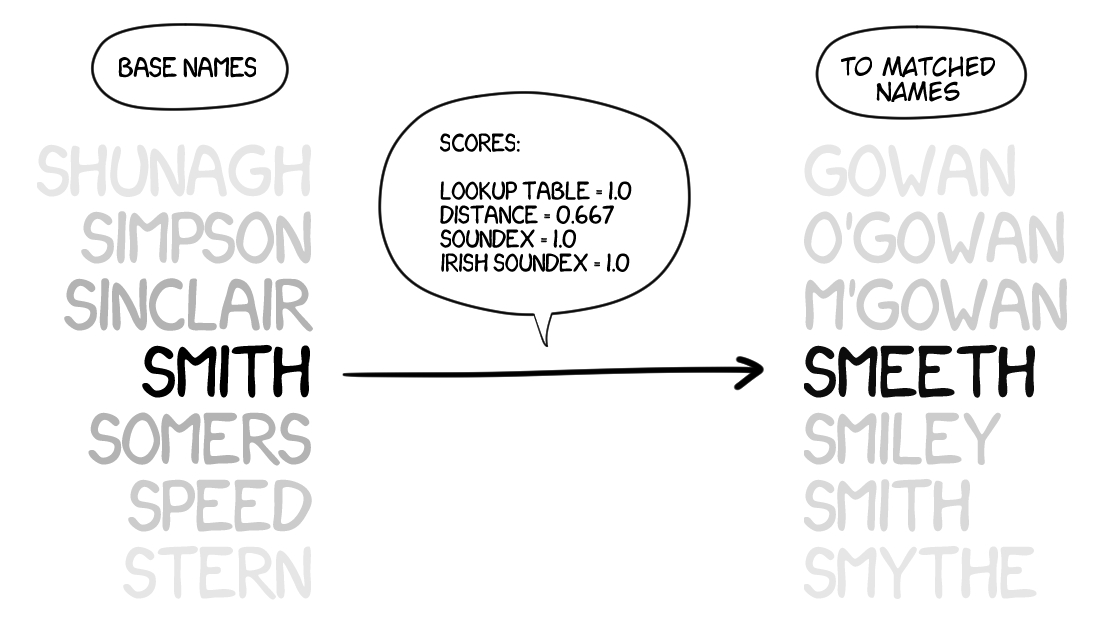
\includegraphics[width=11cm]{gfx/base_tmn}
\caption[\emph{Base name} `SMITH' comparing to \emph{to-match name} `SMEETH'.]{\emph{Base name}
`SMITH' comparing to \emph{to-match name} `SMEETH'. \\
Scores of each matching algorithms
are presented in the bubble above the arrow.}
\label{fig:base_tmn}
\end{figure}

Figure \ref{fig:base_tmn} shows a snapshot of an attempt to match between
\emph{base name} `SMITH' against \emph{to-match name} `SMEETH'.
\emph{Similarity score} for each matching algorithms have been calculated.
And by these scores, we can calculate \emph{overall score} for `SMITH'
and `SMEETH'.

So the next step is to match current \emph{base name}, `SMITH',
against next \emph{to-match name}, `SMILEY'.

Once \emph{base name} `SMITH' completes all \emph{to-match name}\textquotesingle s in their list,
the system then process to the next \emph{base name}, `SOMERS', and start over
the matching process against the whole \emph{to-match name} list again, from
start to the end.

\section{Weighting matching algorithms}
\label{sec:weight}

We realised that, for matching names, each matching algorithms
should not be treated as all the same priority. For example, for Irish names,
it would be better if we favour \emph{Irish soundex} over the
traditional \emph{Soundex}, because it produces more accurate result.

By this idea we also implement \emph{weight} for each matching algorithm.
We will suggest initial values, but also allow client to change these values.
Table \ref{table:weights} states these suggested initial weights.

\begin{table}[H]
  \myfloatalign
  \setlength{\tabcolsep}{0.3cm}
  \begin{tabular}{c c}
    \toprule
    \tableheadline{Matching algorithm} & \tableheadline{Weight} \\
    \midrule
    Levenshtein distance & 1 \\
    Soundex & 3 \\
    Irish soundex & 6 \\
    Lookup table & 10 \\
    \bottomrule
  \end{tabular}
  \caption{Matching algorithm weights.}
  \label{table:weights}
\end{table}

By summarising products of each matching algorithm \emph{similarity score}
and its weight, dividing by sum of all weight, we can obtain
\emph{overall weighted score} (OWS). This sentence can be represented
by equation \ref{eq:ows}.

\begin{equation}
  \begin{gathered}
    OWS = \frac{
      \displaystyle\sum_{i=1}^{n} (s_i \times w_i)
    }{
      \displaystyle\sum_{i=1}^{n} w_i
    }
  \end{gathered}
  \label{eq:ows}
\end{equation}

Where $s$ and $w$ are \emph{similarity score} and weight of
matching algorithm $i$ respectively. $n$ is number of available
matching algorithms.

This \emph{overall weighted score} will represent
each matching and all results will be sorted by this score.
Usage and calculation of this weighting will be described in more detail
in the next section (\ref{sec:actualsys}).

\section{Actual system}
\label{sec:actualsys}

Following our basic idea from previous sections, we then design the
architecture of our system.

Suppose we have two inputs, list of \emph{base names} of length $b$,
and list of \emph{to-match names} of length $t$. We need to
process the matching for $b \times t$ times. We call this single
matching between \emph{base name} and \emph{to-match name}
as \emph{matching cycle}.

In this following figure \ref{fig:overall} we once again show a snapshot
of an attempt to match between \emph{base name} `SMITH'
against \emph{to-match name} `SMEETH'. But now in a \emph{matching cycle} style.

\begin{figure}[H]
\centering
\captionsetup{justification=centering}
\makebox[\textwidth][c]{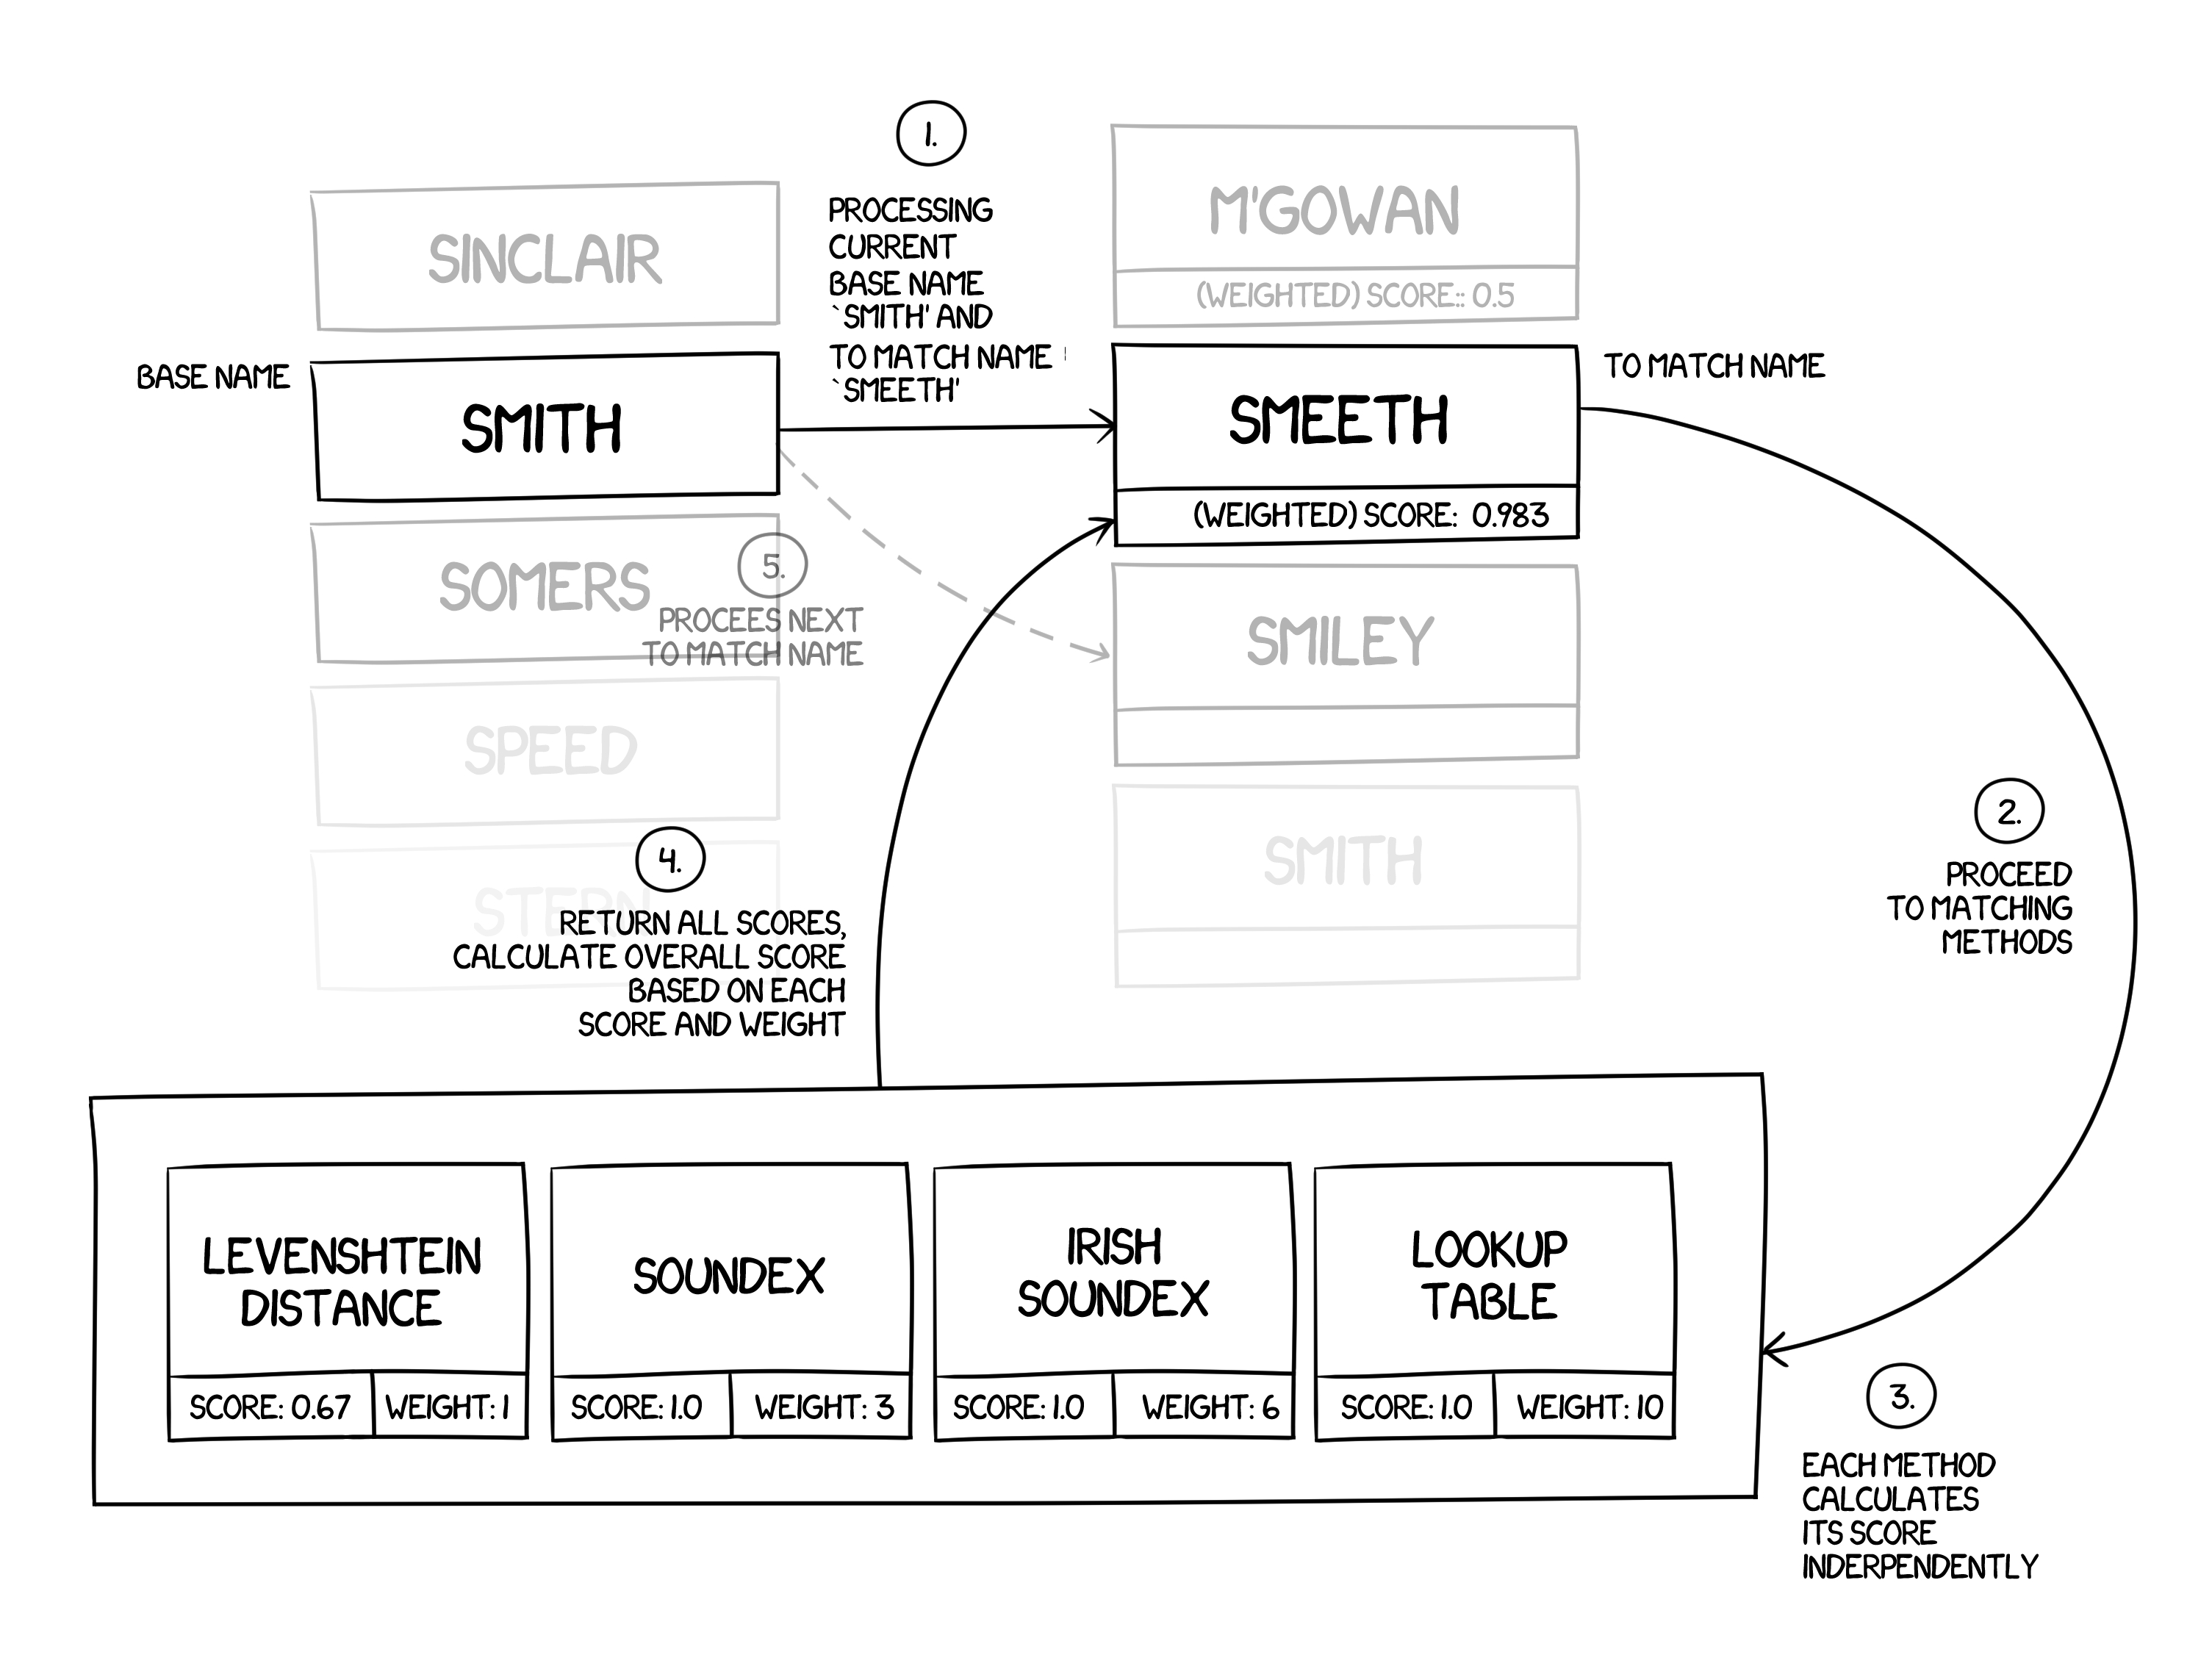
\includegraphics[width=18cm]{gfx/overall}}
\caption{One matching cycle.}
\label{fig:overall}
\end{figure}

One matching cycle consists of 5 steps as shown in figure \ref{fig:overall}.

\begin{enumerate}
  \item Processing current \emph{base name} `SMITH' and \emph{to-match name} `SMEETH'
  \item Proceed to matching algorithms.
  \item Each algorithm calculates its score indepedently.
    \begin{enumerate}
      \item Levenshtein distance between `SMITH' and `SMEETH' is 2
        (1 substitution of \emph{I} to \emph{E} and 1 insertion of \emph{E}).
        So \emph{similarity score} is $(6 - 2) \div 6 = 0.667$ where 6 comes from thelength of the
        longer string, `SMEETH'.

        Weight of this algorithm is 1.

        \textsc{$\therefore$ weighted score = $0.667 \times 1 = 0.667$}
      \item Soundex of both `SMITH' and `SMEETH' are \texttt{S530} so their
        \emph{similarity score} is 1.0.

        Weight of this algorithm is 3.

        \textsc{$\therefore$ weighted score = $1.0 \times 3 = 3.0$}
      \item Irish soundex of both `SMITH' and `SMEETH' are \texttt{S530} so their
        \emph{similarity score} is 1.0.

        Weight of this algorithm is 6.

        \textsc{$\therefore$ weighted score = $1.0 \times 6 = 6.0$}
      \item References between `SMITH' and `SMEETH' is found in the
        Lookup table via group 1897. so their \emph{similarity score} is 1.0

        Weight of this algorithm is 10.

        \textsc{$\therefore$ weighted score = $1.0 \times 10 = 10.0$}
    \end{enumerate}
  \item Return all scores and then calculate \emph{overall weighted score}
    for `SMITH' and `SMEETH'. Sum of the scores is
    $0.667 + 3.0 + 6.0 + 10.0 = 19.667$. Sum of the weights is
    $1 + 3 + 6 + 10 = 20$. Therefore the \emph{overall weighted score} is
    $19.667 \div 20 = 0.983$.
  \item Matching cycle for `SMITH' and `SMEETH' is finished with
    \emph{overall weighted score} 0.983.
    Now the system will proceed to the next \emph{to-match name} `SMILEY'.
    Matching cycles for \emph{base name} `SMITH' will continue until
    the end of \emph{to-match name} list. After that it will start
    matching cycles for \emph{base name} `SOMERS' from the start of
    \emph{to-match names}, and so on.
\end{enumerate}

Once all cycles are fully finished for every \emph{base names} and
\emph{to-match names}, we will get all \emph{overall weighted scores}
ready. So we can sort and present in web interface (section \ref{sec:wi}), or return
as a result in web service (section \ref{sec:ws}).

\section{Thresholding the results}
\label{sec:threshold}

Suppose there are a thousand of \emph{to-match names}, there could be
many irreverent results that are not likely to match each
\emph{base name}. For example \emph{overall weighted scores} of
`SMITH' and `CROMBIE' is just 0.007.

Client may opt-out these irreverent results by specifying
a floating number \emph{threshold}.
Any \emph{to-match name} with \emph{overall weighted scores}
lower than \emph{threshold} will be discarded from the result.

\section{Data flow}
\label{sec:mcv}

In the previous section we describe the essence of this project,
how we use matching algorithms to calculate score of similarity
between two strings. We know how to process the data.
Now in order to make the system becomes useable.
We need to consider two more things.

\begin{itemize}
  \item How to gather inputs from clients.
  \item How to present or return results to clients.
\end{itemize}

From research questions (section \ref{sec:rq}) we mentioned
two ways to communicate with clients, by \emph{web service} and
\emph{web interface}.

Clients who use the system as a web service
will send inputs directly without any medium in between, and will
receive result back in form of agreed format, e.g. \texttt{JSON}.

On the other hand, clients who use the system via web interface
will use a form in a web interface (web page) provided by the system to provide
inputs, and results will be presented in another page
after client submitted the form.

\begin{table}[H]
  \myfloatalign
  \setlength{\tabcolsep}{0.3cm}
  \begin{tabular}{l p{4cm} l}
    \toprule
    \tableheadline{Service type} & \tableheadline{Input source} & \tableheadline{Result format}  \\
    \midrule
    Web service & Web/mobile/desktop application & \texttt{JSON} \\
    \midrule
    Web interface & Provided form & Web page result \\
    \bottomrule
  \end{tabular}
  \caption{Service types and their inputs and results.}
  \label{table:dataflow}
\end{table}

In the next section (\ref{sec:mvc}) we will describe how we
gather inputs and provide results.

\section{MVC}
\label{sec:mvc}

Our system is based on Ruby on Rails, which is a MVC\footnote{Model-View-Controller
\cite[]{mvc}} framework. We will use Rails architecture to encapsulate
our system be these following means.

\begin{description}
  \item[View:] where the form for web interface is implemented.
    It creates a web page with inputs for use to fill in.
    Client can inputs names manually, or upload a file
    containing names. He also can choose whether to use any
    available matching algorithms.

    Inputs from \emph{view} are then passed to \emph{controller}.

    \emph{View} is also responsible in displaying result to
    web interface clients, and generating \texttt{JSON} result
    for web service clients.
  \item[Controller:] receives inputs from different sources,
    inputs from form of web interface style, or direct input from clients
    using web service style. Inputs will be pre-processed, such as
    separating lines from file input, removing white spaces,
    or converting input to upper-case.

    Once inputs are ready, \emph{controller} then passes these inputs
    to \emph{model}, where our matching system lies in.

    After inputs are processed, \emph{controller} receives results
    back from \emph{model}, then \emph{controller} will decide
    which kind of result it needs to return from input source.
    It will then pass results to appropriate \emph{view}.
  \item[Model:] this is where we implement our whole matching system in.
    Model constructs \emph{base names} and \emph{to-match names}
    from received inputs, then invoke matching algorithms, as described
    in section \ref{sec:actualsys}. \emph{Model} will pass results back to
    \emph{controller} after finished.
\end{description}

\begin{figure}[H]
\centering
\captionsetup{justification=centering}
\makebox[\textwidth][c]{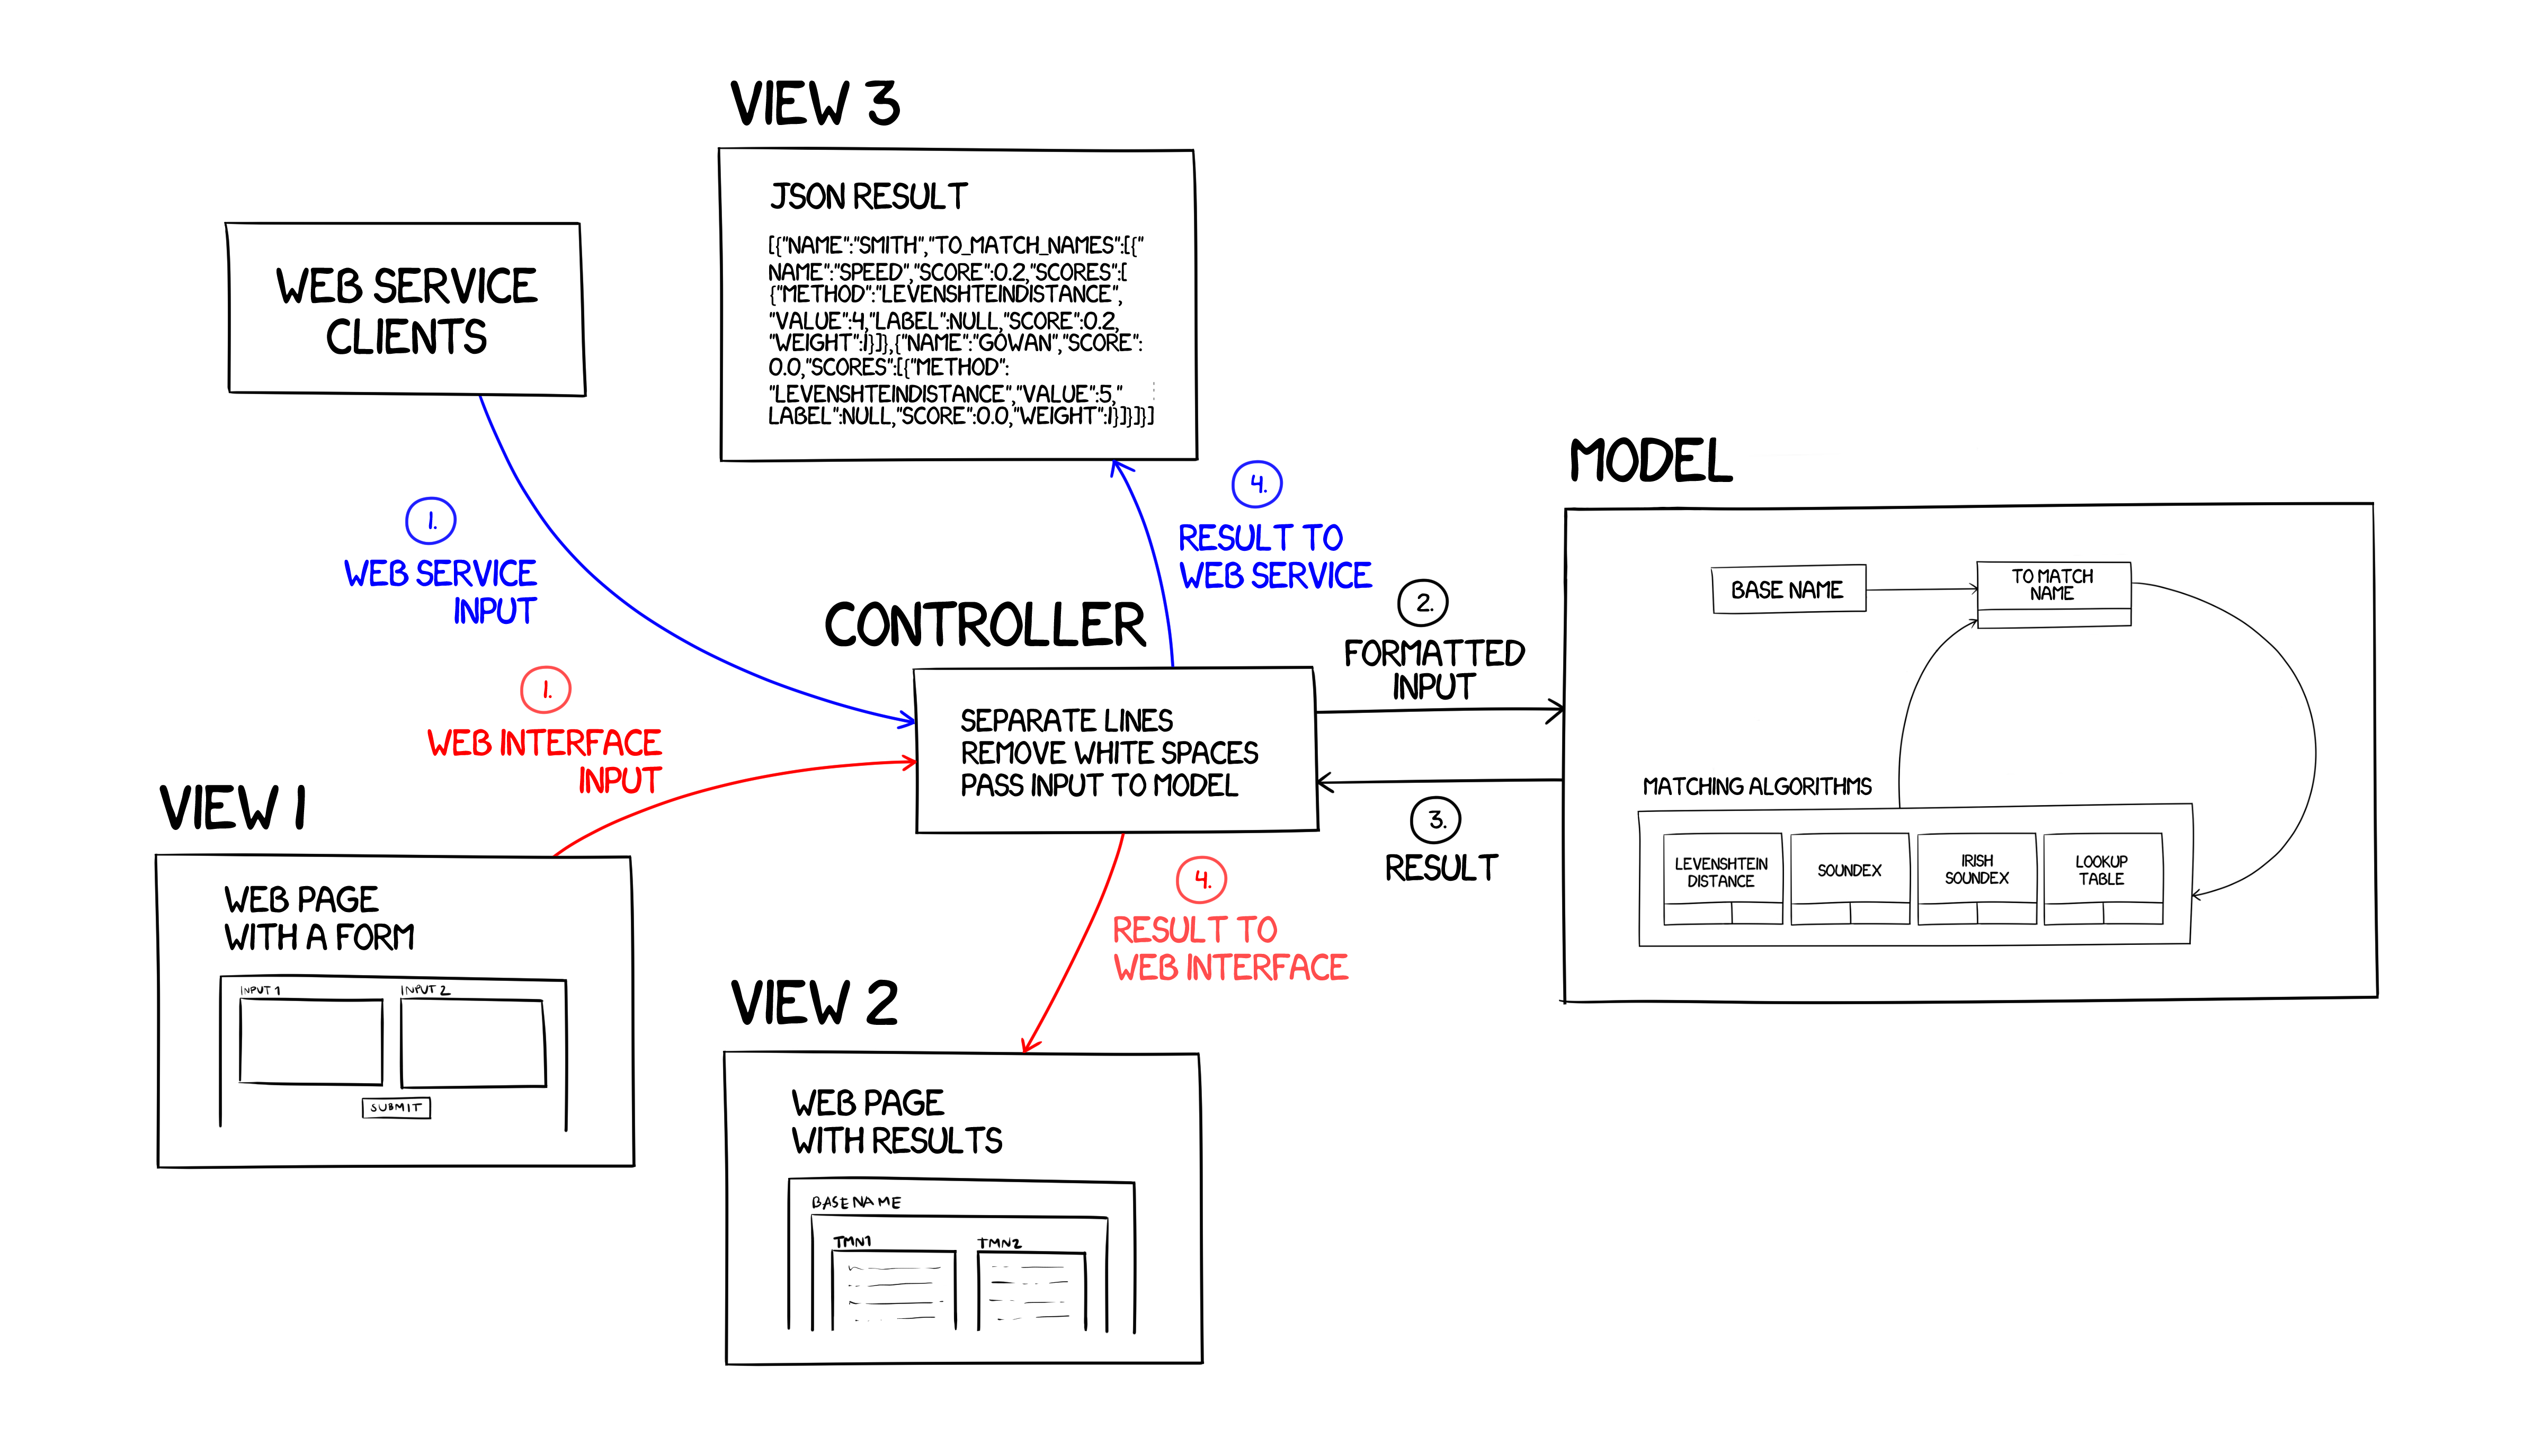
\includegraphics[width=19cm]{gfx/mvc}}
\caption{Data flow from web service client and web interface client.}
\label{fig:mvc}
\end{figure}

\section{Web Service}
\label{sec:ws}

From figure \ref{fig:mvc}, web service clients use the system
by directly pass inputs to the \emph{controller}. Recalling
from previous sessions, all possible inputs to the system
are as follow.

\begin{enumerate}
  \item Base names -- separated by
        new lines\footnote{\texttt{Preferably \textbackslash n} or \texttt{\textbackslash r}, see \url{http://stackoverflow.com/questions/1761051/difference-between-n-and-r}.}.
  \item To-match names -- separated by new lines.
  \item Matching algorithms -- specify needed algorithm names along with its weight (section \ref{sec:weight}).
  \item Threshold (section \ref{sec:threshold}).
  \item Standard list -- will be introduced in section \ref{sec:stdname}.
    Specify \texttt{true}, \texttt{t}, or \texttt{1} to use the standard list.
\end{enumerate}

Currently a preferable format is \texttt{JSON}. In listing \ref{lst:json}
shown a sample \texttt{JSON} input for using web service, let us
call this \texttt{sample.json}.

\begin{minipage}{\linewidth}
\begin{lstlisting}[language={json}, label={lst:json}, caption={\texttt{sample.json}.}]
{
  "base_names":"Smith",
  "to_match_names":"Smythe\r\nO'Gowan",
  "matching_algorithms":{
    "1":{"name":"LookupTable", "weight":"10"},
    "2":{"name":"LevenshteinDistance", "weight":"1"},
    "3":{"name":"Soundex", "weight":"3"},
    "4":{"name":"IrishSoundex", "weight":"6"}
  },
  "threshold":"0",
  "standard_list":""
}
\end{lstlisting}
\end{minipage}

\texttt{sample.json} is an attempt to match between \emph{base name} `SMITH',
and \emph{to-match name} `SMYTHE' and `O\textquotesingle GOWAN'. Using 4 matching
algorithms, and threshold as 0. We will submit this \texttt{sample.json} input
to the system using cURL \cite[]{curl} in command line.

\begin{minipage}{\linewidth}
  \begin{lstlisting}[language={bash}, label={lst:curl}, caption={}]
$ curl -H "Accept: application/json" -H "Content-type: application/json" -X POST -d @sample.json http://localhost:4001/match.json
\end{lstlisting}
\end{minipage}

We use HTTP POST \cite[]{post} to submit \texttt{sample.json} to the web service,
currently running locally, so the \texttt{url} using here is \url{http://localhost:4001/match.json}.
The formatted \texttt{JSON} result is shown in listing \ref{lst:curl2},
note that the result of matching between `SMITH' and `O\textquotesingle GOWAN' is truncated
just for readability.

\begin{lstlisting}[language={json}, label={lst:curl2}, caption={Result from \texttt{sample.json}.}]
[
  {
    "base_name": "SMITH",
    "to_match_names": [
      {
        "to_match_name": "SMYTHE",
        "overall_weighted_score": 0.983,
        "scores": [
          {
            "method": "LookupTable",
            "value": "Matched",
            "label": "1897",
            "score": 1,
            "weight": 10
          },
          {
            "method": "LevenshteinDistance",
            "value": 2,
            "label": null,
            "score": 0.667,
            "weight": 1
          },
          {
            "method": "Soundex",
            "value": "S530 <=> S530",
            "label": null,
            "score": 1,
            "weight": 3
          },
          {
            "method": "IrishSoundex",
            "value": "S530 <=> S530",
            "label": "SMYTHE",
            "score": 1,
            "weight": 6
          }
        ]
      },
      {
        "to_match_name": "O'GOWAN",
        "overall_weighted_score": 0.5,
        ...
\end{lstlisting}

From the results, \emph{overall weighted score} between `SMITH' and `SMYTHE'
is 0.983, higher than `SMITH' and `O\textquotesingle GOWAN' (0.5), so the former is sorted
before the latter.

To generate these results in \texttt{JSON}, we use Jbuilder \cite[]{jbuiler},
a template for generating JSON structures. The template we use is shown
in listing \ref{lst:jbuilder}.

\begin{minipage}{\linewidth}
\begin{lstlisting}[label={lst:jbuilder}, caption={Jbuilder template for generating \texttt{JSON} results.}]
json.array! @matched_names do |matched_name|
  json.base_name matched_name.name

  json.to_match_names do
    json.array! matched_name.to_match_names do |tmn|
      json.to_match_name tmn.name
      json.overall_weighted_score tmn.score

      json.scores do
        json.array! tmn.scores do |s|
          json.method s.class.name
          json.value s.value
          json.label s.label
          json.score s.score
          json.weight s.weight
        end
      end
    end
  end
end
\end{lstlisting}
\end{minipage}


\section{Web Interface}
\label{sec:wi}

Our system provides a web interface with inputs form.
All possible inputs are equivalent to web service as follow.

\begin{enumerate}
  \item Base names -- clients can fill the names in \emph{input 1}, separated
    by new lines. alternatively, clients can also upload a file containing names
    separated by new lines. if the web interface detects that the file input
    is present, direct text input will be discarded.
  \item To-match names -- the same way of \emph{base name}, using \emph{Input 2}.
  \item Matching algorithms -- clients can choose available algorithms
    from the list along with its weight using checkboxes. Uncheck to
    opt-out any algorithms.
  \item Threshold -- clients can specify floating number threshold using input box.
  \item Standard list -- will be introduced in section \ref{sec:stdname}.
    clients can check the checkbox to use the standard list.
\end{enumerate}

\begin{figure}[H]
\centering
\captionsetup{justification=centering}
\makebox[\textwidth][c]{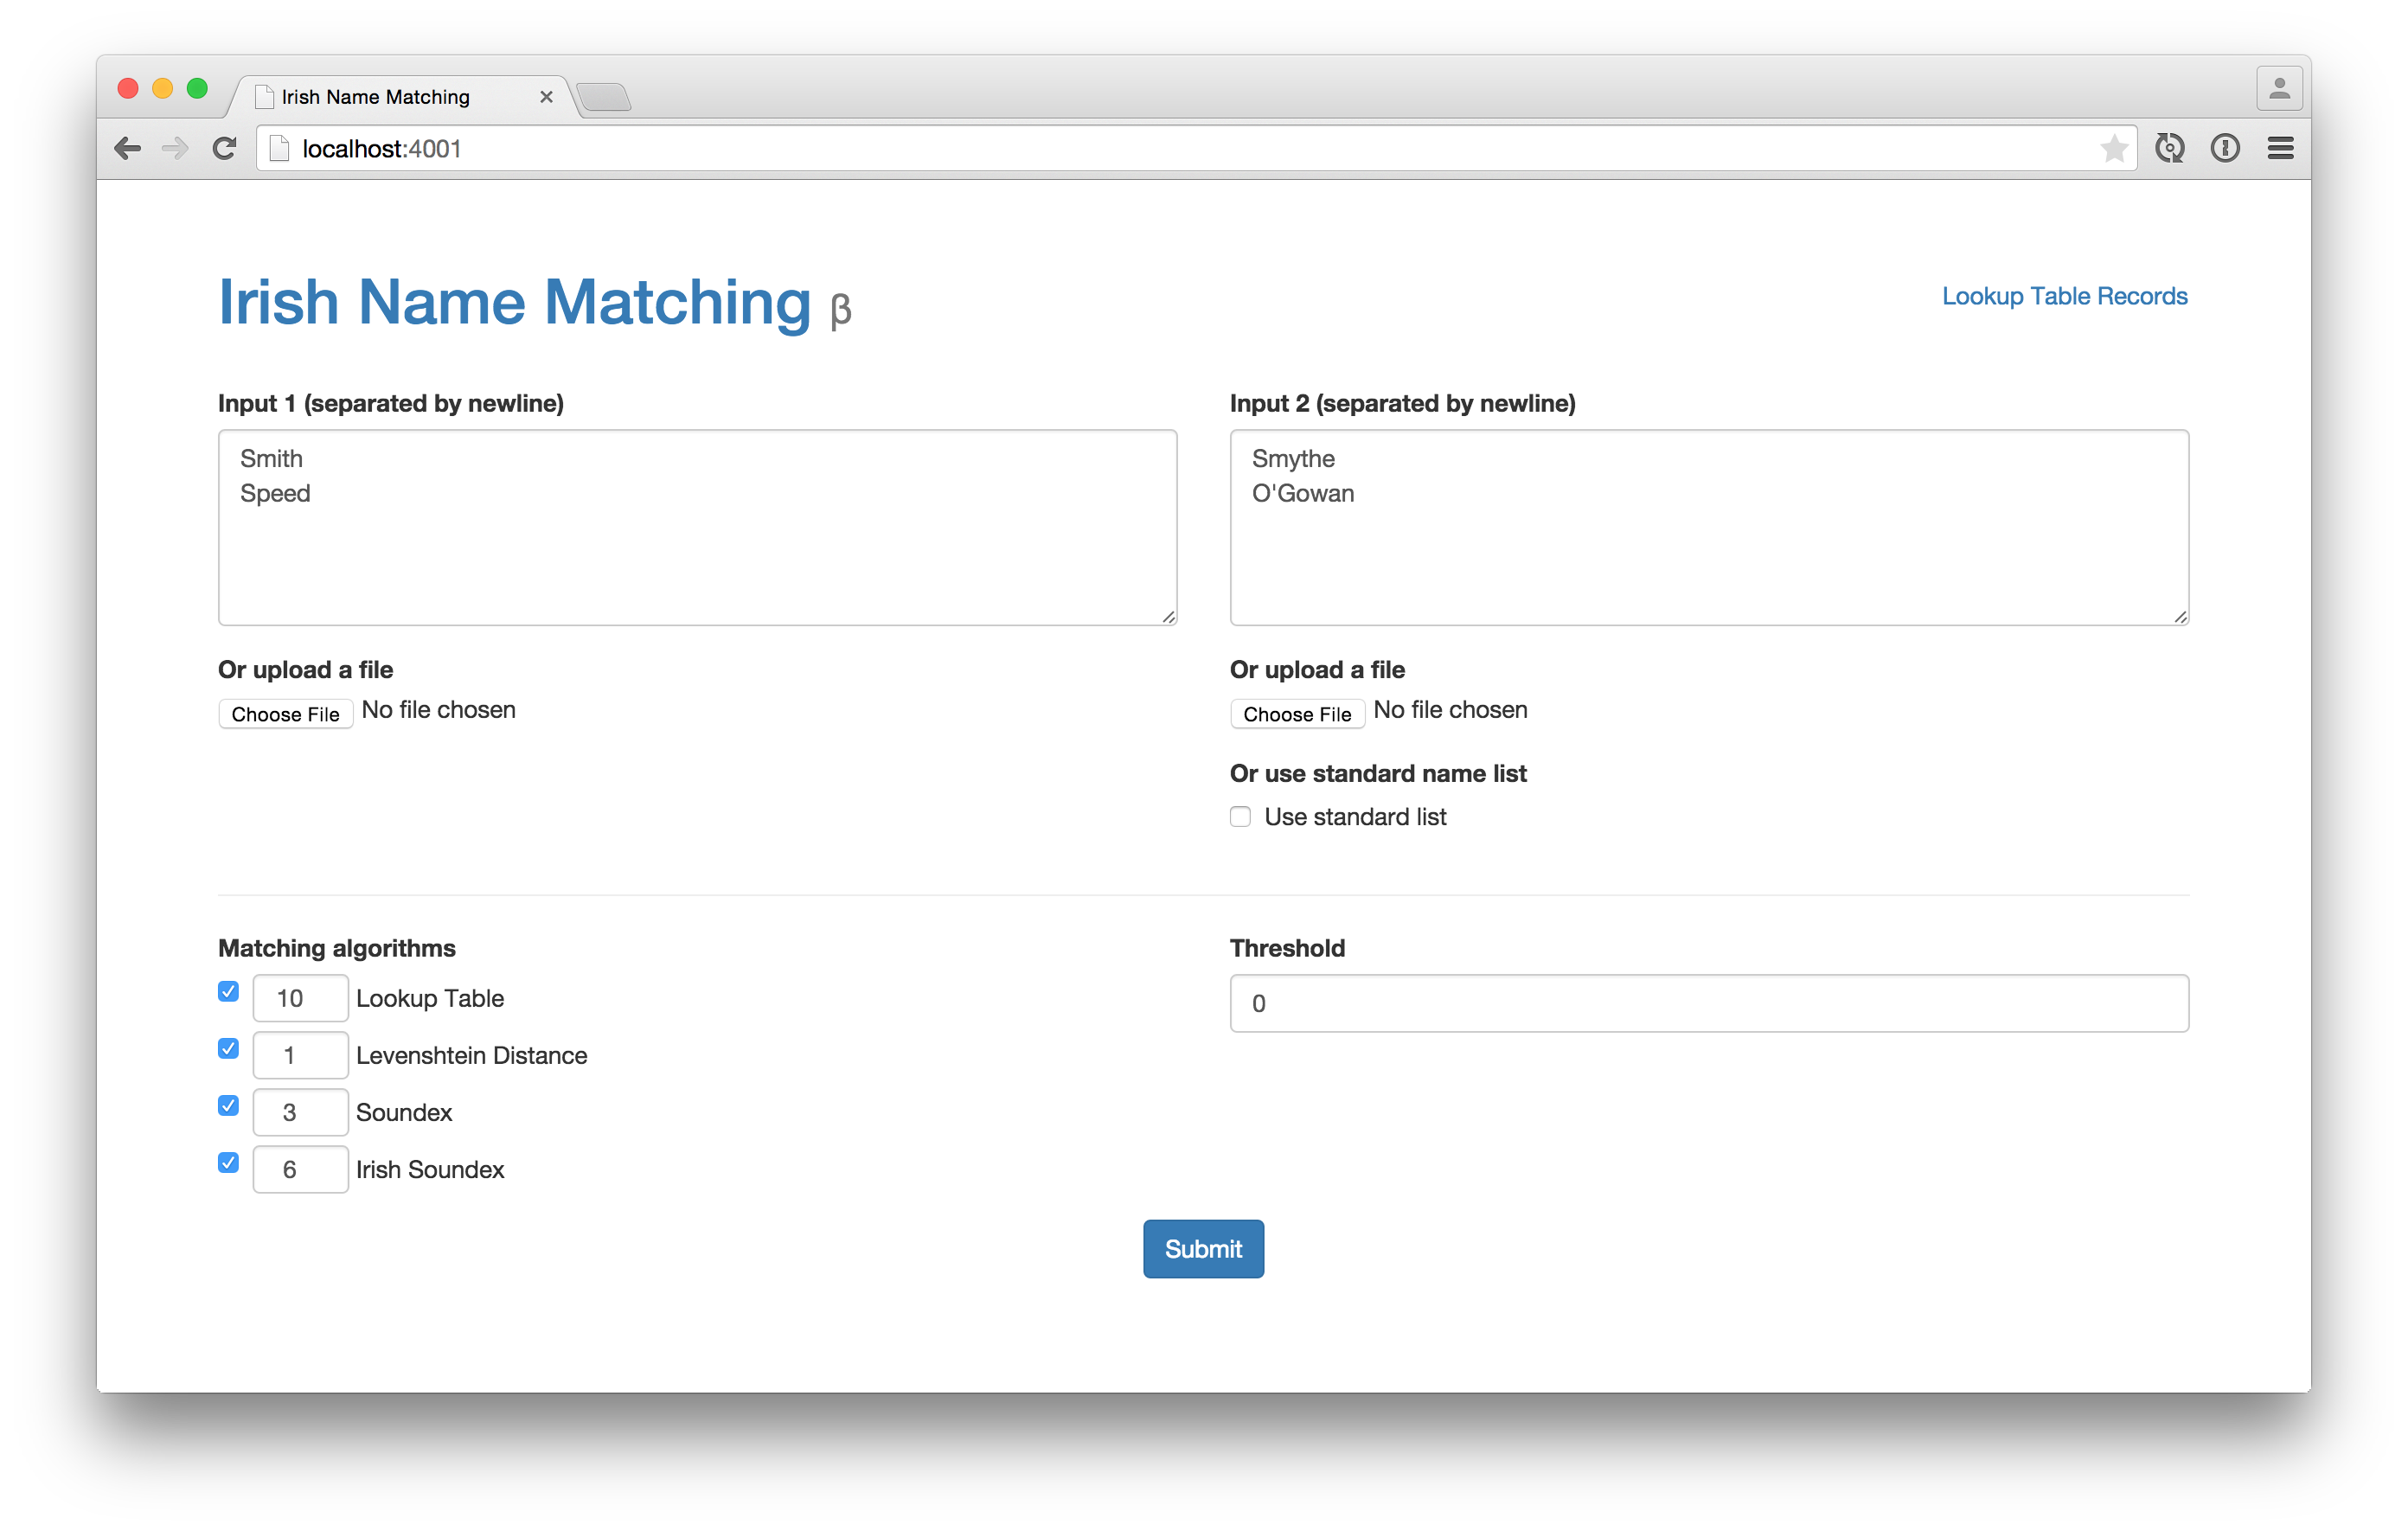
\includegraphics[width=16cm]{gfx/web_interface}}
\caption{Web interface with input forms.}
\label{fig:wi}
\end{figure}

Figure \ref{fig:wi} is an attempt to match between \emph{base name} `SMITH'
and `SPEED', and \emph{to-match name} `SMYTHE' and `O\textquotesingle GOWAN'. Using 4 matching
algorithms, and threshold as 0. After finish filling all inputs client
may press the blue `Submit' button to begin matching.

\begin{figure}[H]
\centering
\captionsetup{justification=centering}
\makebox[\textwidth][c]{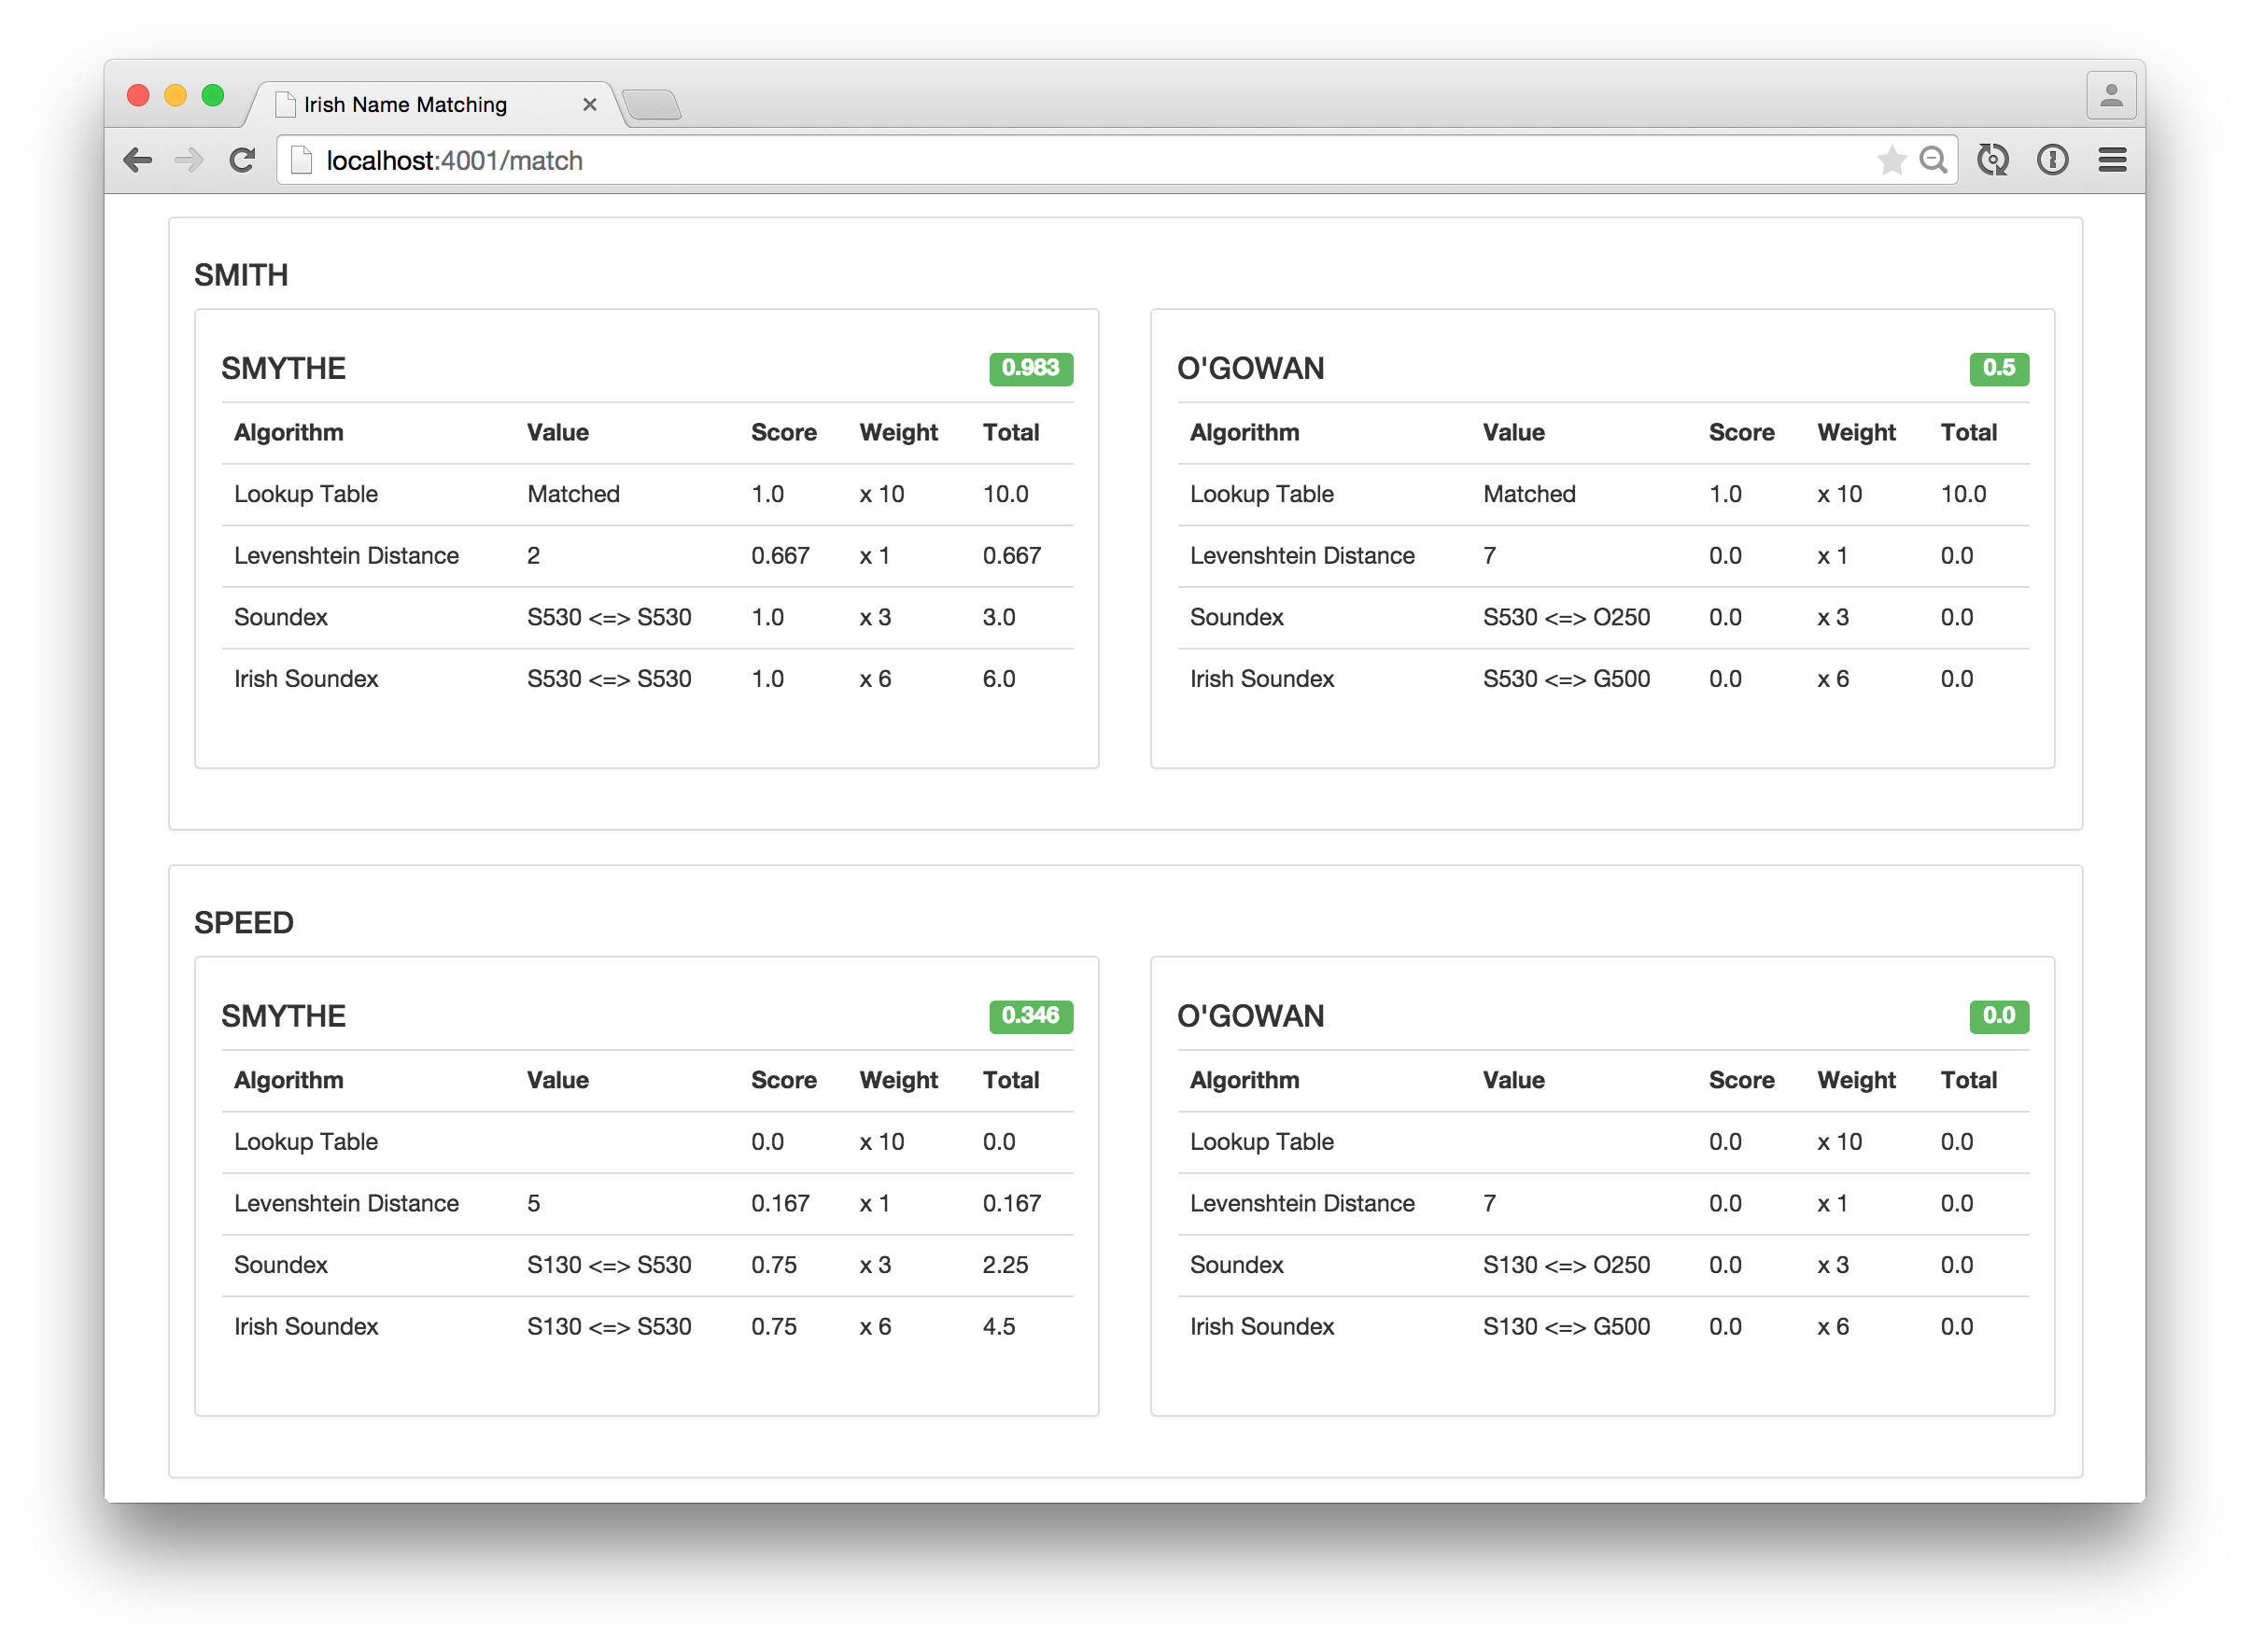
\includegraphics[width=16cm]{gfx/web_interface_result}}
\caption{Web interface results page.}
\label{fig:wi_res}
\end{figure}

Figure \ref{fig:wi_res} shows the web interface result of this matching.
There are two \emph{base names} and two \emph{to-match names}, so the results
are matchings of total $2 \times 2 = 4$ names. Each outer box is results
of matching between each \emph{base names}, with the outer box there
is an inner box containing details of each \emph{to-match names}.

From the results, \emph{overall weighted score}
(each green labelled box) between `SMITH' and `SMYTHE'
is 0.983, higher than `SMITH' and `O\textquotesingle GOWAN' (0.5), so the former is sorted
before the latter.

\chapter{Extending the system}

In this section we show how we design our system to be extensible
in terms of adding new matching algorithms, also using existing
shared methods, or sharing new methods.

\section{Matching algorithms inheritance}

All matching algorithms (chapter \ref{ch:nma}) inherit the same superclass,\\
\texttt{MatchingAlgorithm} (shown in listing \ref{lst:ma_imp}). They all use the same class constructor
(in Ruby, it is called the \emph{initialize} method). To create an instance
of \texttt{MatchingAlgorithm}, current \emph{base name}, \emph{to-match name}
and \emph{weight} are passed as parameters.

We use \emph{The Strategy Pattern}\footnote{\cite[]{hf}, page 24}
as a design pattern. In \texttt{MatchingAlgorithm} the \texttt{cal\_score} method
is declared and also meant to be overridden, so every matching
algorithm needs to override this method using their own matching logic.
Each matching algorithm class will call \texttt{cal\_score}
to calculate its scores.
\texttt{cal\_score} is also private to be only used within the subclasses
themselves.

We also define \texttt{soundex\_distance\_score} method to be shared
between soundex algorithms. Any further shared methods can be declare
here as well.

\texttt{MatchingAlgorithm} class is shown in listing \ref{lst:ma_imp}.

\begin{minipage}{\linewidth}
\begin{lstlisting}[label={lst:ma_imp}, caption={\texttt{MatchingAlgorithm} class.}]
class MatchingAlgorithm
  WEIGHT = 1  # Default weight of every matching algorithm.

  attr_accessor :name,
    :base_name,
    :value,
    :label,
    :score,
    :weight,
    :weighted_score

  def initialize(params = {})
    @name      = params.fetch(:name)
    @base_name = params.fetch(:base_name)
    @weight    = params.fetch(:weight)

    cal_score
    @score = @score.round(3)
    @weighted_score = (@score * @weight).round(3)
  end

  private

  def cal_score
    raise NotImplementedError
  end

  def soundex_distance_score(s1, s2)
    if s1.first != s2.first
      0  # Different category, so they suppose to be completely different
    else
      (s1.size - Text::Levenshtein.distance(s1, s2).to_f ) / s1.size
    end
  end
end
\end{lstlisting}
\end{minipage}

For example of a concrete matching algorithm,
we have already shown some \texttt{cal\_score} overridings. For
\emph{Levenshtein distance} is as in in listing \ref{lst:leven}.
Here we will show whole \texttt{LevenshteinDistance} class,
which is a subclass of \texttt{MatchingAlgorithm}, as in listing \ref{lst:leven_class}.

\begin{minipage}{\linewidth}
\begin{lstlisting}[label={lst:leven_class}, caption={\texttt{LevenshteinDistance} class.}]
class LevenshteinDistance < MatchingAlgorithm
  private

  def cal_score
    @value = Text::Levenshtein.distance(@name, @base_name.name)
    size   = [@name.size, @base_name.name.size].max
    @score = ((size - @value).to_f / size)
  end
end
\end{lstlisting}
\end{minipage}

Also for \emph{Lookup table} is as in listing \ref{lst:lookup}.
Here we will show whole \texttt{LookupTable} class,
which is another subclass of \texttt{MatchingAlgorithm}, as in listing \ref{lst:leven_class}.
Note that \texttt{LookupTable} overrides default \emph{weight}, which
\texttt{LevenshteinDistance} does not.

\begin{minipage}{\linewidth}
\begin{lstlisting}[label={lst:lt_class}, caption={\texttt{LookupTable} class.}]
class LookupTable < MatchingAlgorithm
  WEIGHT = 10  # Overriding default weight.

  private

  def cal_score
    ...
  end
end
\end{lstlisting}
\end{minipage}

\section{Exporting a class method}

When we mentioned soundex implementation in listing \ref{lst:soundex},
we introduced \texttt{self.soundex} method instead of \texttt{cal\_score}.
Defining a method with \texttt{self.} is to create a \emph{class method} \cite[]{classmethod}.
\emph{Class method} can be called directly without creating instance of the class,
it is the same as \emph{static method} in Java. For example as in listing
\ref{lst:classmethod}.

\begin{minipage}{\linewidth}
\begin{lstlisting}[label={lst:classmethod}, caption={Calling class method \emph{Soundex.soundex}.}]
[7] pry(main)> Soundex.soundex('SMITH')
=> "S530"
\end{lstlisting}
\end{minipage}

By defining this method to be a \emph{class method}, it can be reused
in other class as well. In listing \ref{lst:sd_class} we will show whole
\texttt{Soundex} class, which is another subclass of \texttt{MatchingAlgorithm}.

\begin{minipage}{\linewidth}
\begin{lstlisting}[label={lst:sd_class}, caption={\texttt{Soundex} class.}]
class Soundex < MatchingAlgorithm
  WEIGHT = 3

  def self.soundex(name)
    ...
  end

  private

  def self.category(c)
    ...
  end

  def cal_score
    name_soundex      = self.class.soundex(@name)
    base_name_soundex = self.class.soundex(@base_name.name)

    @value = "#{base_name_soundex} <=> #{name_soundex}"
    @score = soundex_distance_score(name_soundex, base_name_soundex)
  end
end
\end{lstlisting}
\end{minipage}

Note that we have already covered \texttt{self.soundex} and \texttt{self.category} implementation
in listing \ref{lst:soundex} and \ref{lst:soundexc} respectively, so both
are truncated for readability. Here we focus on the \texttt{cal\_score} overriding
on \texttt{Soundex} class. The use of \texttt{self.class.soundex} in \texttt{cal\_score}
refers to \texttt{Soundex.soundex}. And \texttt{soundex\_distance\_score}
is defined in \texttt{MatchingAlgorithm}.

As for Irish soundex, it also contains its own \texttt{self.soundex}
\emph{class method}. But this \texttt{self.soundex} also calls \texttt{Soundex.soundex}
to use original soundex code, as in listing \ref{lst:is_call_s} (extracted from
\texttt{IrishSoundex.soundex} implementation, listing \ref{lst:irishsoundex}).

\begin{minipage}{\linewidth}
\begin{lstlisting}[label={lst:is_call_s}, caption={\texttt{IrishSoundex.soundex} calls to \texttt{Soundex.soundex}.}]
# Call to traditional soundex.
return {
  :label => name,
  :soundex => Soundex.soundex(name)
}
\end{lstlisting}
\end{minipage}

In listing \ref{lst:is_class} we will show whole \texttt{IrishSoundex} class,
which is another subclass of \texttt{MatchingAlgorithm}.

\begin{minipage}{\linewidth}
  \begin{lstlisting}[label={lst:is_class}, caption={\texttt{IrishSoundex} class.}]
class IrishSoundex < MatchingAlgorithm
  WEIGHT = 6

  def self.soundex(name)
    ..
  end

  private

  def cal_score
    name_soundex      = self.class.soundex(@name)
    base_name_soundex = self.class.soundex(@base_name.name)

    @value = "#{base_name_soundex[:soundex]} <=> #{name_soundex[:soundex]}"
    @label = name_soundex[:label]
    @score = soundex_distance_score(name_soundex[:soundex], base_name_soundex[:soundex])
  end
end
\end{lstlisting}
\end{minipage}

Note that we have already covered \texttt{self.soundex} implementation
in listing \ref{lst:irishsoundex}, so it is truncated for readability.
Here we focus on the \texttt{cal\_score} overriding
on \texttt{IrishSoundex} class. The use of \texttt{self.class.soundex} in \texttt{cal\_score}
refers to \texttt{IrishSoundex.soundex}. And \texttt{soundex\_distance\_score}
is defined in \texttt{MatchingAlgorithm}.


\section{Implementing new matching algorithms}


% \cleardoublepage % Empty page before the start of the next part

%------------------------------------------------

% \ctparttext{}

\part{The Outcome}

\chapter{Conclusion}
\label{ch:conclusion}

\lipsum[1]

\section{Outcome}

\lipsum[1]

\section{Encountered problem}

\lipsum[2]

\section{Future works}

\lipsum[3]

\chapter{Conclusion}
\label{ch:conclusion}

\section{Outcome}

\section{Encountered problem}

\section{Future works}


% \cleardoublepage % Empty page before the start of the next part

%------------------------------------------------

% \ctparttext{You can put some informational part preamble text here. Illo principalmente su nos. Non message \emph{occidental} angloromanic da. Debitas effortio simplificate sia se, auxiliar summarios da que, se avantiate publicationes via. Pan in terra summarios, capital interlingua se que. Al via multo esser specimen, campo responder que da. Le usate medical addresses pro, europa origine sanctificate nos se.} % Text on the Part 2 page describing the content in Part 2
%
% \part{The Showcase}
%
% % Chapter 1

\chapter{Introduction} % Chapter title

\label{ch:introduction_s} % For referencing the chapter elsewhere, use \autoref{ch:introduction}

%----------------------------------------------------------------------------------------

This template for \LaTeX\ has two goals:
\begin{enumerate}
\item Provide students with an easy-to-use template for their Master's or PhD thesis (though it might also be used by other types of authors for reports, books, etc.).
\item Provide a classic, high-quality typographic style that is inspired by ``\emph{The Elements of Typographic Style}''.
\marginpar{\myTitle \myVersion}
\end{enumerate}

The bundle is configured to run with a \emph{full} MiK\TeX\ or \TeX Live installation right away and, therefore, it uses only freely available fonts.

People interested only in the nice style and not the whole bundle can now use the style stand-alone via the file \texttt{classicthesis.sty}. This works now also with ``plain'' \LaTeX.

As of version 3.0, \texttt{classicthesis} can also be easily used with \mLyX\footnote{\url{http://www.lyx.org}} thanks to Nicholas Mariette and Ivo Pletikosi\'c. The \mLyX\ version of this manual will contain more information on the details.

This should enable anyone with a basic knowledge of \LaTeXe\ or \mLyX\ to produce beautiful documents without too much effort. In the end, this is my overall goal: more beautiful documents, especially theses, as I am tired of seeing so many ugly ones.

The whole template and the used style is released under the \textsmaller{GNU} General Public License.

If you like the style then I would appreciate a postcard:
\begin{center}
Andre Miede \\
Detmolder Strasse 32 \\
31737 Rinteln \\
Germany
\end{center}

\noindent The postcards I received so far are available at:
\begin{center}
 \url{http://postcards.miede.de}
\end{center}
\marginpar{A well-balanced line width improves the legibility of the text. That's what typography is all about, right?} So far, many theses, some books, and several other publications have been typeset successfully with it. If you are interested in some typographic details behind it, enjoy Robert Bringhurst's wonderful book.

\paragraph{Important Note:} Some things of this style might look unusual at first glance, many people feel so in the beginning. However, all things are intentionally designed to be as they are, especially these:
\begin{itemize}
\item No bold fonts are used. Italics or spaced small caps do the job quite well.
\item The size of the text body is intentionally shaped like it is. It supports both legibility and allows a reasonable amount of information to be on a page. And, no: the lines are not too short.
\item The tables intentionally do not use vertical or double rules. See the documentation for the \texttt{booktabs} package for a nice discussion of this topic.\footnote{To be found online at \\ \url{http://www.ctan.org/tex-archive/macros/latex/contrib/booktabs/}.}
\item And last but not least, to provide the reader with a way easier access to page numbers in the table of contents, the page numbers are right behind the titles. Yes, they are \emph{not} neatly aligned at the right side and they are \emph{not} connected with dots that help the eye to bridge a distance that is not necessary. If you are still not convinced: is your reader interested in the page number or does she want to sum the numbers up?
\end{itemize}

\noindent Therefore, please do not break the beauty of the style by changing these things unless you really know what you are doing! Please.

%----------------------------------------------------------------------------------------

\section{Organization}
A very important factor for successful thesis writing is the organization of the material. This template suggests a structure as the following:
\begin{itemize}
\marginpar{You can use these margins for summaries of the text body\dots}
\item\texttt{Chapters/} is where all the ``real'' content goes in separate files such as \texttt{Chapter01.tex} etc.
\item\texttt{FrontBackMatter/} is where all the stuff goes that surrounds the ``real'' content, such as the acknowledgments, dedication, etc.
\item\texttt{gfx/} is where you put all the graphics you use in the thesis. Maybe they should be organized into subfolders depending on the chapter they are used in, if you have a lot of graphics.
\item\texttt{Bibliography.bib}: the Bib\TeX\ database to organize all the references you might want to cite.
\item\texttt{classicthesis.sty}: the style definition to get this awesome look and feel. Bonus: works with both \LaTeX\ and \textsc{pdf}\LaTeX\dots and \mLyX.
\item\texttt{ClassicThesis.tcp} a \TeX nicCenter project file. Great tool and it's free!
\item\texttt{ClassicThesis.tex}: the main file of your thesis where all the content gets bundled together.
\item\texttt{classicthesis-config.tex}: a central place to load all nifty packages that are used. In there, you can also activate backrefs in order to have information in the bibliography about where a source was cited in the text (\ie, the page number).

\emph{Make your changes and adjustments here.} This means that you specify here the options you want to load \texttt{classicthesis.sty} with. You also adjust the title of your thesis, your name, and all similar information here. Refer to \autoref{sec:custom} for more information.

This had to change as of version 3.0 in order to enable an easy transition from the ``basic'' style to \mLyX.
\end{itemize}

\noindent In total, this should get you started in no time.

%----------------------------------------------------------------------------------------

\section{Style Options}\label{sec:options}

There are a couple of options for \texttt{classicthesis.sty} that allow for a bit of freedom concerning the layout: \marginpar{\dots or your supervisor might use the margins for some comments of her own while reading.}
\begin{itemize}
\item General:
\begin{itemize}
\item\texttt{drafting}: prints the date and time at the bottom of each page, so you always know which version you are dealing with. Might come in handy not to give your Prof. that old draft.
\end{itemize}

\item Parts and Chapters:
\begin{itemize}
\item\texttt{parts}: if you use Part divisions for your document, you should choose this option. (Cannot be used together with \texttt{nochapters}.)

\item\texttt{nochapters}: allows to use the look-and-feel with classes that do not use chapters, \eg, for articles. Automatically turns off a couple of other options: \texttt{eulerchapternumbers}, \texttt{linedheaders}, \texttt{listsseparated}, and \texttt{parts}.

\item\texttt{linedheaders}: changes the look of the chapter headings a bit by adding a horizontal line above the chapter title. The chapter number will also be moved to the top of the page, above the chapter title.
\end{itemize}

\item Typography:
\begin{itemize}
\item\texttt{eulerchapternumbers}: use figures from Hermann Zapf's Euler math font for the chapter numbers. By default, old style figures from the Palatino font are used.

\item\texttt{beramono}: loads Bera Mono as typewriter font. (Default setting is using the standard CM typewriter font.)
\item\texttt{eulermath}: loads the awesome Euler fonts for math. (Palatino is used as default font.)

\item\texttt{pdfspacing}: makes use of pdftex' letter spacing capabilities via the \texttt{microtype} package.\footnote{Use \texttt{microtype}'s \texttt{DVIoutput} option to generate DVI with pdftex.} This fixes some serious issues regarding math formul\ae\ etc. (\eg, ``\ss'') in headers.

\item\texttt{minionprospacing}: uses the internal \texttt{textssc} command of the \texttt{MinionPro} package for letter spacing. This automatically enables the \texttt{minionpro} option and overrides the \texttt{pdfspacing} option.
\end{itemize}

\item Table of Contents:
\begin{itemize}
\item\texttt{tocaligned}: aligns the whole table of contents on the left side. Some people like that, some don't.

\item\texttt{dottedtoc}: sets pagenumbers flushed right in the table of contents.

\item\texttt{manychapters}: if you need more than nine chapters for your document, you might not be happy with the spacing between the chapter number and the chapter title in the Table of Contents. This option allows for additional space in this context. However, it does not look as ``perfect'' if you use \verb|\parts| for structuring your document.
\end{itemize}

\item Floats:
\begin{itemize}
\item\texttt{listings}: loads the \texttt{listings} package (if not already done) and configures the List of Listings accordingly.

\item\texttt{floatperchapter}: activates numbering per chapter for all floats such as figures, tables, and listings (if used).

\item\texttt{subfig}(\texttt{ure}): is passed to the \texttt{tocloft} package to enable compatibility with the \texttt{subfig}(\texttt{ure}) package. Use this option if you want use classicthesis with the \texttt{subfig} package.

\end{itemize}

\end{itemize}

\noindent The best way to figure these options out is to try the different possibilities and see, what you and your supervisor like best.

In order to make things easier in general, \texttt{classicthesis-config.tex} contains some useful commands that might help you.

%----------------------------------------------------------------------------------------

\section{Customization}\label{sec:custom}

This section will give you some hints about how to adapt \texttt{classicthesis} to your needs.

The file \texttt{classicthesis.sty} contains the core functionality of the style and in most cases will be left intact, whereas the file \texttt{classic\-thesis-config.tex} is used for some common user customizations.

The first customization you are about to make is to alter the document title, author name, and other thesis details. In order to do this, replace the data in the following lines of \texttt{classicthesis-config.tex:}\marginpar{Modifications in \texttt{classic\-thesis-config.tex}
}

\begin{lstlisting}[frame=lt]
\newcommand{\myTitle}{A Classic Thesis Style\xspace}
\newcommand{\mySubtitle}{An Homage to ...\xspace}
\newcommand{\myDegree}{Doktor-Ingenieur (Dr.-Ing.)\xspace}
\end{lstlisting}

Further customization can be made in \texttt{classicthesis-config.tex} by choosing the options to \texttt{classicthesis.sty} (see~\autoref{sec:options}) in a line that looks like this:

\begin{lstlisting}[frame=lt]
\PassOptionsToPackage{eulerchapternumbers,listings,drafting, pdfspacing, subfig,beramono,eulermath,parts}{classicthesis}

\end{lstlisting}

If you want to use backreferences from your citations to the pages they were cited on, change the following line from:
\begin{lstlisting}[breaklines=false,frame=lt]
\setboolean{enable-backrefs}{false}
\end{lstlisting}
to
\begin{lstlisting}[breaklines=false,frame=lt]
\setboolean{enable-backrefs}{true}
\end{lstlisting}

Many other customizations in \texttt{classicthesis-config.tex} are possible, but you should be careful making changes there, since some changes could cause errors.

Finally, changes can be made in the file \texttt{classicthesis.sty}, \marginpar{Modifications in \texttt{classicthesis.sty}} although this is mostly not designed for user customization. The main change that might be made here is the text-block size, for example, to get longer lines of text.

%----------------------------------------------------------------------------------------

\section{Issues}\label{sec:issues}
This section will list some information about problems using \texttt{classic\-thesis} in general or using it with other packages.

Beta versions of \texttt{classicthesis} can be found at the following Google code repository:
\begin{center}
\url{http://code.google.com/p/classicthesis/}
\end{center}

\noindent There, you can also post serious bugs and problems you encounter.

\subsection*{Compatibility with the \texttt{glossaries} Package}
If you want to use the \texttt{glossaries} package, take care of loading it with the following options:
\begin{verbatim}
\usepackage[style=long,nolist]{glossaries}
\end{verbatim}

\noindent Thanks to Sven Staehs for this information.

\subsection*{Compatibility with the (Spanish) \texttt{babel} Package}
Spanish languages need an extra option in order to work with this template:
\begin{verbatim}
\usepackage[spanish,es-lcroman]{babel}
\end{verbatim}

\noindent Thanks to an unknown person for this information (via Google Code issue reporting).

\subsection*{Compatibility with the \texttt{pdfsync} Package}
Using the \texttt{pdfsync} package leads to linebreaking problems with the \texttt{graffito} command. Thanks to Henrik Schumacher for this information.

%----------------------------------------------------------------------------------------

\section{Future Work}
So far, this is a quite stable version that served a couple of people well during their thesis time. However, some things are still not as they should be. Proper documentation in the standard format is still missing. In the long run, the style should probably be published separately, with the template bundle being only an application of the style. Alas, there is no time for that at the moment\dots it could be a nice task for a small group of \LaTeX nicians.

Please do not send me email with questions concerning \LaTeX\ or the template, as I do not have time for an answer. But if you have comments, suggestions, or improvements for the style or the template in general, do not hesitate to write them on that postcard of yours.

%----------------------------------------------------------------------------------------

\section{License}
\paragraph{GNU General Public License:} This program is free software; you can redistribute it and/or modify it under the terms of the \textsmaller{GNU} General Public License as published by the Free Software Foundation; either version 2 of the License, or (at your option) any later version.

This program is distributed in the hope that it will be useful, but \emph{without any warranty}; without even the implied warranty of \emph{merchantability} or \emph{fitness for a particular purpose}. See the \textsmaller{GNU} General Public License for more details.

% % Chapter 2

\chapter{Examples} % Chapter title

\label{ch:examples} % For referencing the chapter elsewhere, use \autoref{ch:examples}

%----------------------------------------------------------------------------------------

\lipsum[1]

%----------------------------------------------------------------------------------------

\section{A New Section}

\lipsum[2]

Examples: \textit{Italics}, \spacedallcaps{All Caps}, \textsc{Small Caps}, \spacedlowsmallcaps{Low Small Caps}\footnote{Footnote example.}.

%------------------------------------------------

\subsection{Test for a Subsection}

\graffito{Note: The content of this chapter is just some dummy text.}
\lipsum[3-5]

%------------------------------------------------

\subsection{Autem Timeam}

\lipsum[6]

%----------------------------------------------------------------------------------------

\section{Another Section in This Chapter}

\lipsum[7]

Sia ma sine svedese americas. Asia representantes un nos, un altere membros qui.\footnote{De web nostre historia angloromanic.} Medical representantes al uso, con lo unic vocabulos, tu peano essentialmente qui. Lo malo laborava anteriormente uso.

\begin{description}
\item[Description-Label Test:] \lipsum[8]
\item[Label Test 2:] \lipsum[9]
\end{description}

\noindent This statement requires citation.

%------------------------------------------------

\subsection{Personas Initialmente}

\lipsum[10]

\subsubsection{A Subsubsection}
\lipsum[11]

\paragraph{A Paragraph Example} \lipsum[12]

\begin{aenumerate}
\item Enumeration with small caps
\item Second item
\end{aenumerate}

\noindent Another statement requiring citation but this time with text after the citation.

\begin{table}
\myfloatalign
\begin{tabularx}{\textwidth}{Xll} \toprule
\tableheadline{labitur bonorum pri no} & \tableheadline{que vista}
& \tableheadline{human} \\ \midrule
fastidii ea ius & germano &  demonstratea \\
suscipit instructior & titulo & personas \\
\midrule
quaestio philosophia & facto & demonstrated \\
\bottomrule
\end{tabularx}
\caption[Autem timeam deleniti usu id]{Autem timeam deleniti usu id.}
\label{tab:example}
\end{table}

\enlargethispage{2cm}

%------------------------------------------------

\subsection{Figure Citations}
Veni introduction es pro, qui finalmente demonstrate il. E tamben anglese programma uno. Sed le debitas demonstrate. Non russo existe o, facite linguistic registrate se nos. Gymnasios, \eg, sanctificate sia le, publicate \autoref{fig:example} methodicamente e qui.

Lo sed apprende instruite. Que altere responder su, pan ma, \ie, signo studio. \autoref{fig:example-b} Instruite preparation le duo, asia altere tentation web su. Via unic facto rapide de, iste questiones methodicamente o uno, nos al.

\begin{figure}[bth]
\myfloatalign
\subfloat[Asia personas duo.]
{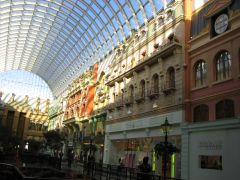
\includegraphics[width=.45\linewidth]{gfx/example_1}} \quad
\subfloat[Pan ma signo.]
{\label{fig:example-b}
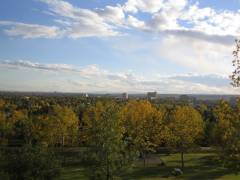
\includegraphics[width=.45\linewidth]{gfx/example_2}} \\
\subfloat[Methodicamente o uno.]
{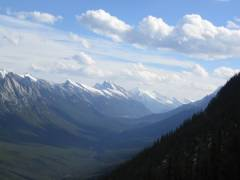
\includegraphics[width=.45\linewidth]{gfx/example_3}} \quad
\subfloat[Titulo debitas.]
{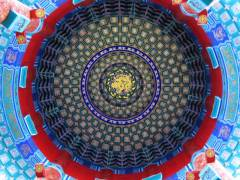
\includegraphics[width=.45\linewidth]{gfx/example_4}}
\caption[Tu duo titulo debitas latente]{Tu duo titulo debitas latente.}\label{fig:example}
\end{figure}

% % Chapter 3

\chapter{Math Test Chapter} % Chapter title

\label{ch:mathtest} % For referencing the chapter elsewhere, use \autoref{ch:mathtest}

%----------------------------------------------------------------------------------------

\lipsum[13]

%----------------------------------------------------------------------------------------

\section{Some Formulas}

Due to the statistical nature of ionisation energy loss, large fluctuations can occur in the amount of energy deposited by a particle traversing an absorber element\footnote{Examples taken from Walter Schmidt's great gallery: \\ \url{http://home.vrweb.de/~was/mathfonts.html}}.  Continuous processes such as multiple scattering and energy loss play a relevant role in the longitudinal and lateral development of electromagnetic and hadronic showers, and in the case of sampling calorimeters the measured resolution can be significantly affected by such fluctuations in their active layers.  The description of ionisation fluctuations is characterised by the significance parameter $\kappa$, which is proportional to the ratio of mean energy loss to the maximum allowed energy transfer in a single collision with an atomic electron: \graffito{You might get unexpected results using math in chapter or section heads. Consider the \texttt{pdfspacing} option.}
\begin{equation}
\kappa =\frac{\xi}{E_{\mathrm{max}}} %\mathbb{ZNR}
\end{equation}
$E_{\mathrm{max}}$ is the maximum transferable energy in a single collision with an atomic electron.
\[E_{\mathrm{max}} =\frac{2 m_{\mathrm{e}} \beta^2\gamma^2 }{1 + 2\gamma m_{\mathrm{e}}/m_{\mathrm{x}} + \left ( m_{\mathrm{e}} /m_{\mathrm{x}}\right)^2}\ ,\]

where $\gamma = E/m_{\mathrm{x}}$, $E$ is energy and $m_{\mathrm{x}}$ the mass of the incident particle, $\beta^2 = 1 - 1/\gamma^2$ and $m_{\mathrm{e}}$ is the electron mass. $\xi$ comes from the Rutherford scattering cross section and is defined as:
\begin{eqnarray*} \xi  = \frac{2\pi z^2 e^4 N_{\mathrm{Av}} Z \rho
\delta x}{m_{\mathrm{e}} \beta^2 c^2 A} =  153.4 \frac{z^2}{\beta^2}
\frac{Z}{A}
\rho \delta x \quad\mathrm{keV},
\end{eqnarray*}
where

\begin{tabular}{ll}
$z$ & charge of the incident particle \\
$N_{\mathrm{Av}}$ & Avogadro's number \\
$Z$ & atomic number of the material \\
$A$ & atomic weight of the material \\
$\rho$ & density \\
$ \delta x$ & thickness of the material \\
\end{tabular}

$\kappa$ measures the contribution of the collisions with energy transfer close to $E_{\mathrm{max}}$.  For a given absorber, $\kappa$ tends towards large values if $\delta x$ is large and/or if $\beta$ is small.  Likewise, $\kappa$ tends towards zero if $\delta x $ is small and/or if $\beta$ approaches $1$.

The value of $\kappa$ distinguishes two regimes which occur in the description of ionisation fluctuations:

\begin{enumerate}
\item A large number of collisions involving the loss of all or most of the incident particle energy during the traversal of an absorber.

As the total energy transfer is composed of a multitude of small energy losses, we can apply the central limit theorem and describe the fluctuations by a Gaussian distribution. This case is applicable to non-relativistic particles and is described by the inequality $\kappa > 10 $ (\ie, when the mean energy loss in the absorber is greater than the maximum energy transfer in a single collision).

\item Particles traversing thin counters and incident electrons under any conditions.

The relevant inequalities and distributions are $ 0.01 < \kappa < 10 $, Vavilov distribution, and $\kappa < 0.01 $, Landau distribution.
\end{enumerate}

%----------------------------------------------------------------------------------------

\section{Various Mathematical Examples}

If $n > 2$, the identity \[t[u_1,\dots,u_n] = t\bigl[t[u_1,\dots,u_{n_1}], t[u_2,\dots,u_n] \bigr]\] defines $t[u_1,\dots,u_n]$ recursively, and it can be shown that the alternative definition \[t[u_1,\dots,u_n] = t\bigl[t[u_1,u_2],\dots,t[u_{n-1},u_n]\bigr]\] gives the same result.


% \cleardoublepage % Empty page before the start of the next part

%----------------------------------------------------------------------------------------
% THESIS CONTENT - APPENDICES
%----------------------------------------------------------------------------------------

\appendix

\part{Appendix} % New part of the thesis for the appendix

% Appendix A

\chapter{Appendix Test}

%----------------------------------------------------------------------------------------

\lipsum[13-14]

%----------------------------------------------------------------------------------------

\section{Appendix Section Test}
\lipsum[15]

\graffito{More dummy text}

%----------------------------------------------------------------------------------------


\begin{table}
\myfloatalign
\begin{tabularx}{\textwidth}{Xll}
\toprule
\tableheadline{labitur bonorum pri no} & \tableheadline{que vista} & \tableheadline{human} \\
\midrule
fastidii ea ius & germano &  demonstratea \\
suscipit instructior & titulo & personas \\
\midrule
quaestio philosophia & facto & demonstrated \\
\bottomrule
\end{tabularx}
\caption[Autem usu id]{Autem usu id.}
\label{tab:moreexample}
\end{table}

\section{Another Appendix Section Test}

Your own text.

\begin{lstlisting}[float,caption=A floating example]
for i:=maxint to 0 do
begin
{ do nothing }
end;
\end{lstlisting}

\subsection{Sub}

\lipsum[11]
 % Appendix A

%----------------------------------------------------------------------------------------
% POST-CONTENT THESIS PAGES
%----------------------------------------------------------------------------------------

\cleardoublepage% Bibliography

\label{app:bibliography} % Reference the bibliography elsewhere with \autoref{app:bibliography}

\manualmark
\markboth{\spacedlowsmallcaps{\bibname}}{\spacedlowsmallcaps{\bibname}}
\refstepcounter{dummy}

\addtocontents{toc}{\protect\vspace{\beforebibskip}} % Place the bibliography slightly below the rest of the document content in the table of contents
\addcontentsline{toc}{chapter}{\tocEntry{\bibname}}

\bibliographystyle{unsrtnat}

\bibliography{Bibliography}
 % Bibliography

% \cleardoublepage% Colophon (a brief description of publication or production notes relevant to the edition)

\pagestyle{empty}

\hfill

\vfill

\pdfbookmark[0]{Colophon}{colophon}

\section*{Colophon}

This document was typeset using the typographical look-and-feel \texttt{classicthesis} developed by Andr\'e Miede. The style was inspired by Robert Bringhurst's seminal book on typography ``\emph{The Elements of Typographic Style}''. \texttt{classicthesis} is available for both \LaTeX\ and \mLyX: 

\begin{center}
\url{http://code.google.com/p/classicthesis/}
\end{center}

\noindent Happy users of \texttt{classicthesis} usually send a real postcard to the author, a collection of postcards received so far is featured here: 

\begin{center}
\url{http://postcards.miede.de/}
\end{center}
 
\bigskip

\noindent\finalVersionString % Colophon
%
% \cleardoublepage% Declaration

\refstepcounter{dummy}
\pdfbookmark[0]{Declaration}{declaration} % Bookmark name visible in a PDF viewer

\chapter*{Declaration} % Declaration section text

\thispagestyle{empty}

I declare that the dissertation report and code for
``Web service for 19\textsuperscript{th} century Irish personal name matching''
submitted for assessment is my own work except where credit
is explicitly given to others by citation or acknowledgement.
This work was accomplished during the current academic year except
where otherwise stated.

In submitting this project report to the Maynooth University,
I hereby give permission for it to be made available for use
in accordance with the regulations of the University Library.
I also give permission for the title and abstract to be published
and for copies of the report to be made and supplied at cost
to any bona fide library or research worker,
and to be made available on the World Wide Web.
In addition, I retain the copyright to this work.

\bigskip

% \noindent\textit{\myLocation, \myTime}
% \smallskip

\begin{flushright}
\begin{tabular}{m{5cm}}
\begin{center}

\includegraphics[width=5cm]{gfx/signature}\\
\end{center}
\\ \hline
\centering\myName, \today \\
\end{tabular}
\end{flushright}
 % Declaration

%----------------------------------------------------------------------------------------

\end{document}
